\documentclass[12pt]{article}

\usepackage{float}
\usepackage{color}
\usepackage{caption}
\usepackage[margin=1in]{geometry}
\usepackage{amsmath}
\usepackage{xspace}
\usepackage{setspace}
\usepackage{lineno}
\usepackage{graphicx}
\usepackage{natbib}
\usepackage{subfigure}
\usepackage{longtable}
\usepackage{multirow}

\begin{document}
\doublespacing
\linenumbers

\newcommand{\Lik}{\ensuremath{\mathcal{L}}\xspace}
\newcommand{\selac}{\emph{SelAC}\xspace}
\newcommand{\selacDMS}{\emph{SelAC}+DMS\xspace}
\newcommand{\phydms}{\emph{phydms}\xspace}
\newcommand{\gy}{\emph{GY94}\xspace}
\newcommand{\ecoli}{\textit{E. coli}\xspace}
\newcommand{\PC}{physicochemical\xspace}

\newcommand{\beginsupplement}{%
  %%% commands for getting SM pages and figures labeled with S
  %% different than with other .cls
  \setcounter{section}{19} %appendix environment set in .cls file.  Set this to 19 to get an 'S' for figures
  \setcounter{page}{1}
  \renewcommand{\thepage}{S\arabic{page}} %this works

  \setcounter{table}{0}
  \renewcommand{\thetable}{S\arabic{table}}%
  \setcounter{figure}{0}
  \renewcommand{\thefigure}{S\arabic{figure}}%
}


\noindent RH: LANDERER ET AL.--- Estimating site specific selection
% put in your own RH (running head)
% for POVs the RH is always POINT OF VIEW
\bigskip
\medskip
\begin{center}

% Insert your title:
\noindent{\Large \bf Phylogenetic model of stabilizing selection is more informative about site specific selection than extrapolation from laboratory estimates.}
\bigskip

\noindent{C\textsc{EDRIC} ~{L\textsc{ANDERER}}$^{1,2,*}$,
B\textsc{RIAN} C.~ {O\textsc{MEARA}}$^{1,2}$,
\textsc{AND}
M\textsc{ICHAEL} A.~{G\textsc{ILCHRIST}}$^{1,2}$}

\end{center}

\vfill

{\small
\noindent$^{1}$Department of Ecology \& Evolutionary Biology, University of Tennessee, Knoxville, TN 37996-1610\\
\noindent$^{2}$National Institute for Mathematical and Biological Synthesis, Knoxville, TN 37996-3410\\
\noindent$^{*}$Corresponding author. E-mail:~cedric.landerer@gmail.com
}

\vfill
\centerline{Version dated: \today}
\vfill
\newpage

\begin{abstract}
Here we examine the adequacy of experimentally inferred site specific selection for amino acids to inform phylogenetic inferences of sequence evolution.
Previous work has shown that laboratory estimates of selection can improve model fit but did not assess their adequacy.
We assess the adequacy of experimentally inferred site specific selection using DMS to inform phylogenetic models.
We use the $\beta$-lactamse TEM for which empirical estimates of site specific selection on amino acids are readily available.
We compare our results to \selac, a new phylogenetic model of stabilizing selection.
Using simulations to assess model adequacy, we find that experimentally inferred selection does not adequately reflect evolution in the wild.
In contrast, \selac improves model fit over models informed by experimentally inferred selection and provides higher model adequacy.
We demonstrate the capability of \selac by estimating site specific genetic load of the observed TEM variants.

\end{abstract}
\newpage

\section*{Introduction}

Numerous attempts to incorporat selection into phylogenetic models have been made.
Early models focused on the influence of selection on the substitution rate and fixation probability between a resident and a mutant introduced into a population\citep{GoldmanAndYang1994, MuseAndGaut1994, thorne1996}.
These models however, lack site specific equilibrium frequencies.
The importance of site specific equilibrium frequencies has long been noted \citep{felsenstein1981, gojobori1983}.
\citet{HalpernAndBruno1998} first introduced a model to incorporate site specific equilibrium frequencies of amino acids.
However, they had to concede that their model was too parameter rich and therefore intractable for biological data sets without additional simplifying assumptions.
More recent models incorporating site specific equilibrium frequencies still require a large number of parameter to be estimated from the sequence data \citep{LartillotAndPhilippe2004,le2008,wang2008,holder2008,wu2013,tamuri2014}.
Other approaches treat site specific selection as a random effect \citep{rodrigue2010,rodrigue2013,rodrigue2014}.
A full parameterization of site specific equilibrium frequencies for amino acids requires $19\times L$ parameters were $L$ is the length of the sequence.
It is therefore an attractive option to utilize laboratory experiments to empirically estimate site specific strength of selection on amino acids and infer their equilibrium frequencies \citep{bloom2014, thyagarajan2014, bloom2017}.

Incorporating empirical estimates of site specific strength of selection on amino acids has important advantages.
Individual amino acid site along the protein show differences in evolutionary rates, and strong preferences for amino acids \citep{HalpernAndBruno1998, ashenberg2013, echave2016}.
The usage of site specific selection acknowledges the heterogeneity in selection and amino acid preferences along the protein sequence \citep{hilton2017}.
Empirical estimates of site specific selection reduce the number of parameters that have to be estimated from the data, making it applicable for smaller data sets and allowing for the fitting of more complex models.
There are, however, also shortcomings.
Deep mutation scanning (DMS) has recently been recently used to generate comprehensive site specific estimates of the strength of selection on amino acids \citep{Fowler2014}.
The ability to estimate site specific strength of selection on amino acids allows to estimte site specific amino acid preferences and the genetic load a mutation introduces at a particular site\citep{bloom2014,firnberg2014,stiffler2016}.
The quality of empirical estimates from DMS, however, depends on many factors including the initial library of mutants and the applied selection \citep{FirnbergAndOstermeier2012}.
Mutation libraries have to be extensive and therefore produce a heterogeneous population of competing organsims usually not found in nature.
In addition, estimates of selection can only be obtained for fast growing organisms that can be manipulated under laboratory conditions.
This is a severe limitation of experimentally informed models as many organism can not be cultivated under laboratory conditions or have long generation times.

Even in the cases were empirical estimates of site specific selection on amino acids can be obtained, their applicability for phylogenetic reconstruction is quastionable.
In this study, we assess the adequacy of experimentally inferred site specific selection using DMS to inform phylogenetic models and offer an alternative approach to deterimine site specific selection on amino aicds.
We use site specific estimates of selection on amino acids for the $\beta$-lactamase TEM from \citet{stiffler2016}.
We fitted $227$ nucleotide and codon models using IQTree and compared their model fits to site specific models of stabilizing selection with (\phydms, \selacDMS) and without (\selac) experimentally determined site specific selection coefficients on amino acids \citep{nguyen2015,hilton2017,beaulieu2018}.
We find that experimentally inferred selection, while improving model fit, does not adequately reflect observed wild type sequences.
In contrast, \selac \citep{beaulieu2018} a mechanistic phylogenetic model of stabilizing selection rooted in first principles with site specific equilibrium frequencies improves model fit, and better reflects evolution in the wild.
Because \selac assumes stabilizing selection and that the distance of two amino acids in \PC space affects substitution probabilities it is able to infer the optimal amino acid at a site and reduce the number of site specific parameters from $19\times L$ to $L$.

\section*{Results}

\subsection*{Site Specific Stabilizing Selection on Amino Acids Improves Model Fit}
We compared \phydms \citep{hilton2017} and \selac \citep{beaulieu2018}, models of site specific stabilizing selection on amino acids, to $227$ other codon and nucleotide models.
We fitted all models to 49 observed sequences of the $\beta$-lactamase TEM.
The \phydms and \selac models with site specific selection on amino acids improved model fits by $366$ and $934$ AICc units, respectively, over codon or nucleotide models without site specific selection (Table \ref{tab:AIC}).
In addition, \selac outperformed the experimentally informed model \phydms by $562$ to $568$ AICc units, depending whether site specific selection on amino acids was inferred by \selac or experimentally informed.

\selac utilizes a hierarchical model and estimates 263 site specific parameters, $\sim5\%$ of the $19\times L = 4997$ parameters necessary to fully describe the site specific selection on amino acids.
In contrast, \phydms does not infer any site specific parameters, but utilizes site specific selection on amino acids estimated from deep mutation scanning experiments.
We fixed the optimal amino acid at each site to the experimentally determined one in \selac and refitted the model to the 49 TEM sequences (\selacDMS).
Incorporating site specific selection on amino acids estimated from deep mutation scanning experiments into \selac (\selacDMS) yields a similar AICc value to \selac without that information.
We incorporated the experimentally inferred site specific amino acids by estimating the 

However, \selacDMS is favored by AICc.
This is solely due to a decrease in the number of parameters estimated, as the model log-likelihood ($\log(\Lik)$) worsens from $-1498$ to $-1768$ (Table \ref{tab:AIC}).
$263$ of the $374$ parameters estimated are the discrete optimal amino acid state at each site. 
However, it is unclear if discrete parameters contribute to the Kullback-Leibler divergence like continous parameters do and have to be penelaized like such.
Therefore, the number of parameter for \selac is reported conservatively as the number of unique site patterns in the TEM alignment is only 27 which would yield a total number of $1383$ parameters (96 edge length, 15 mutation/selection parameters, and 27 optimal amion acids).
This however would likely be an under estimate of the number of parameteres estimated and the true number of parameters remains unclear at this point due to the inherent non-independence of the underlying data and the descrete nature of the optimized parameters.

\begin{table}
  \centering
  \begin{tabular}{lrrrrrr}
    Model		& $\log(\Lik)$ & n & AIC & $\Delta$AIC & AICc & $\Delta$AICc\\ \hline 
    \selacDMS 		& -1768 & 111& 3758& 14	& 3760  & 0\\
    \selac		& -1498 & 374& 3744&  0	& 3766  & 6 \\
    \phydms 		& -2061 & 102& 4326& 582& 4328 & 568\\
    SYM+R2 		& -2230 & 102& 4663& 919& 4694 & 934 \\
    GY+F1X4+R2 		& -2243 & 102& 4690& 946& 4821 & 1061 \\
  \end{tabular}
  \caption{Model selection, shown are the three models of stabilizing site specific amino acid selection (\selac, \selacDMS, \phydms) and the best performing codon and nucleotide model. 
  Reported are the log-likelihood ($\log(\Lik)$), the number of parameters estiamted $n$ including edge length, AIC, $\Delta$AIC, AICc, and $\Delta$AICc values.
  See Table \ref{tab:AIC} for all models tested.}
  \label{tab:AIC}
\end{table}

\begin{figure}[H]
     \centering
	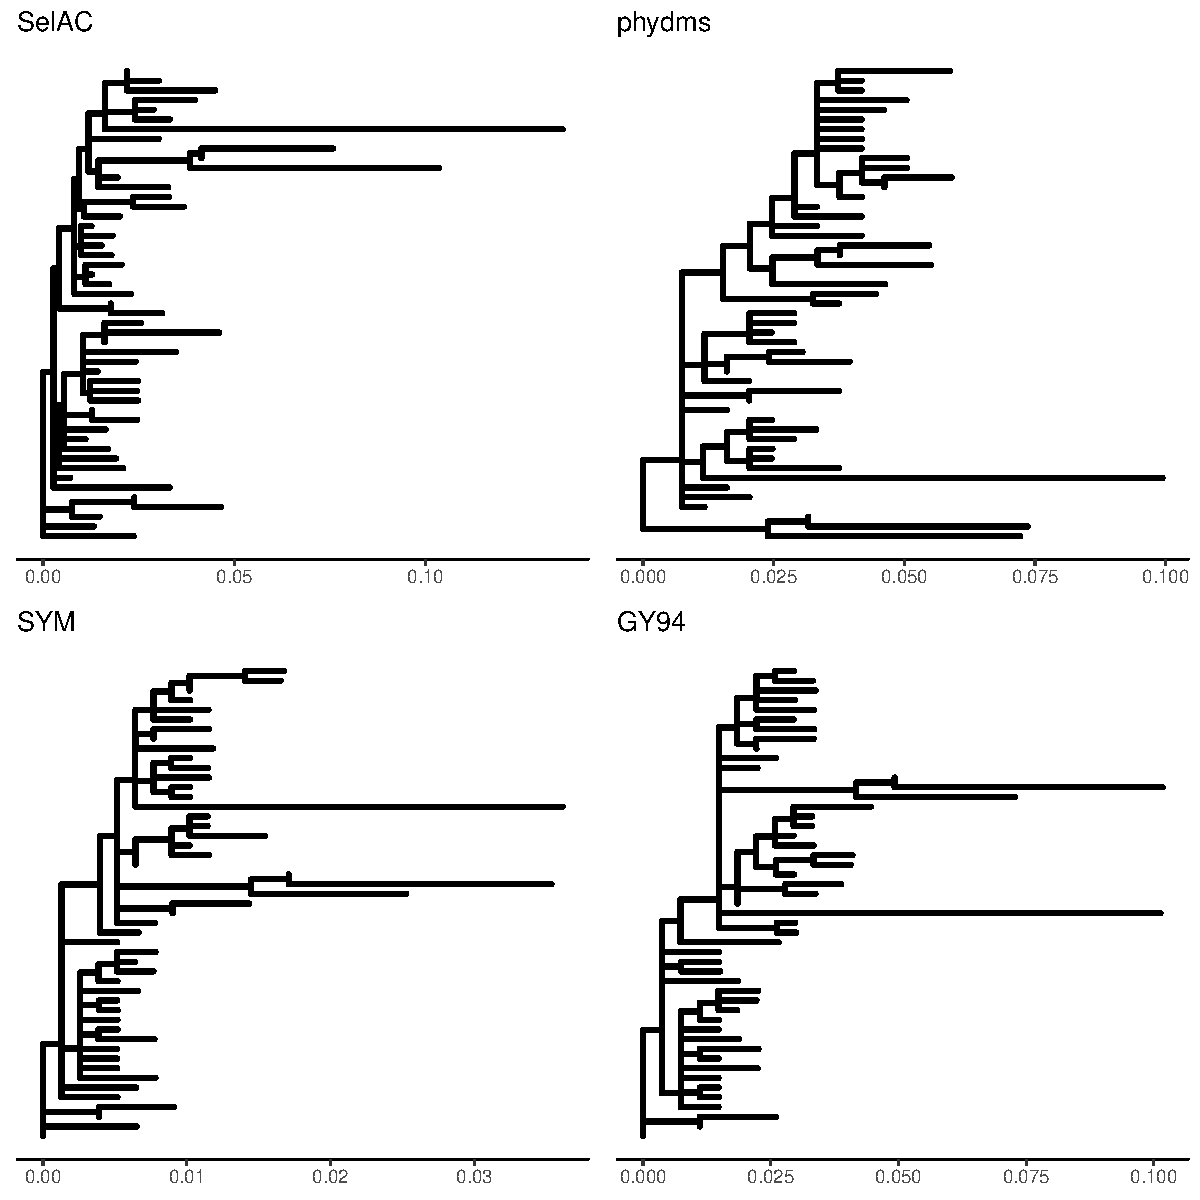
\includegraphics[width=\textwidth]{img/phy_TEM2016.pdf}
	\caption{Phylogenies resulting from \selac, \selacDMS, \phydms, and \gy. As \selac is currently to slow for the inference of tomopogies, the topology for the \selac phylogenies was inferred using the codon model of \citet{KosiolEtAl07}.}
	\label{fig:phylo}
\end{figure}

We observe differences in the topology between model fits.
The \selac model is currently too slow to estimate the topology, therefore the topology was estimated using the codon model of \citet{KosiolEtAl07}.
At this point, it is therefore unclear if the difference in topology can be attributes to the experimentally inferred selection on amino acids.
We find that the best codon model (\gy) \citep{GoldmanAndYang1994} is outperformed by several nucleotide model e.g. \emph{SYM} \citep{zharkikh1994}.
This could be an indication that negative frequency dependent selection like it is modeled in \gy is not appropriate for TEM \citep{GoldmanAndYang1994,beaulieu2018}.
Figure \ref{fig:phylo} shows that the estimated phylogenetic trees shift from long terminal branches (\selac) to longer internal branches (\phydms).
While the \selac model fit shows $84 \%$ of all evolution happening at the tips, this reduces to $79 \%$ in the \selacDMS model fit, and $77 \%$ in the \phydms and \gy model fits.
All models produce polytomies but their location differs between models.
The largest polytomies appear in the experimentally informed phylogenies of \phydms.
The position of the sequences with the longest branches differ between \selac and \phydms.


\subsection*{Laboratory Inferences Inconsistent with Observed Sequences.}
The improved model fits with phydms relative to classical nucleotide and codon models are, however, deceiving.
The site specific selection inferred by the deep mutation scanning experiment is inconsistent with the observed TEM sequences.
We find that the sequence of selectively favored amino acids has only $52 \%$ sequence similarity with the observed consensus sequence (Figure \ref{fig:sim_seqs_cons}).
In addition, assuimg the site specific selection estimated by DMS, the observed TEM sequences represent an unexpectedly high genetic load.
%This is in contrast to the $99 \%$ of sequence similarity with the sequence of selectively favored amino acids estimated by \selac.

\begin{figure}[H]
     \centering
	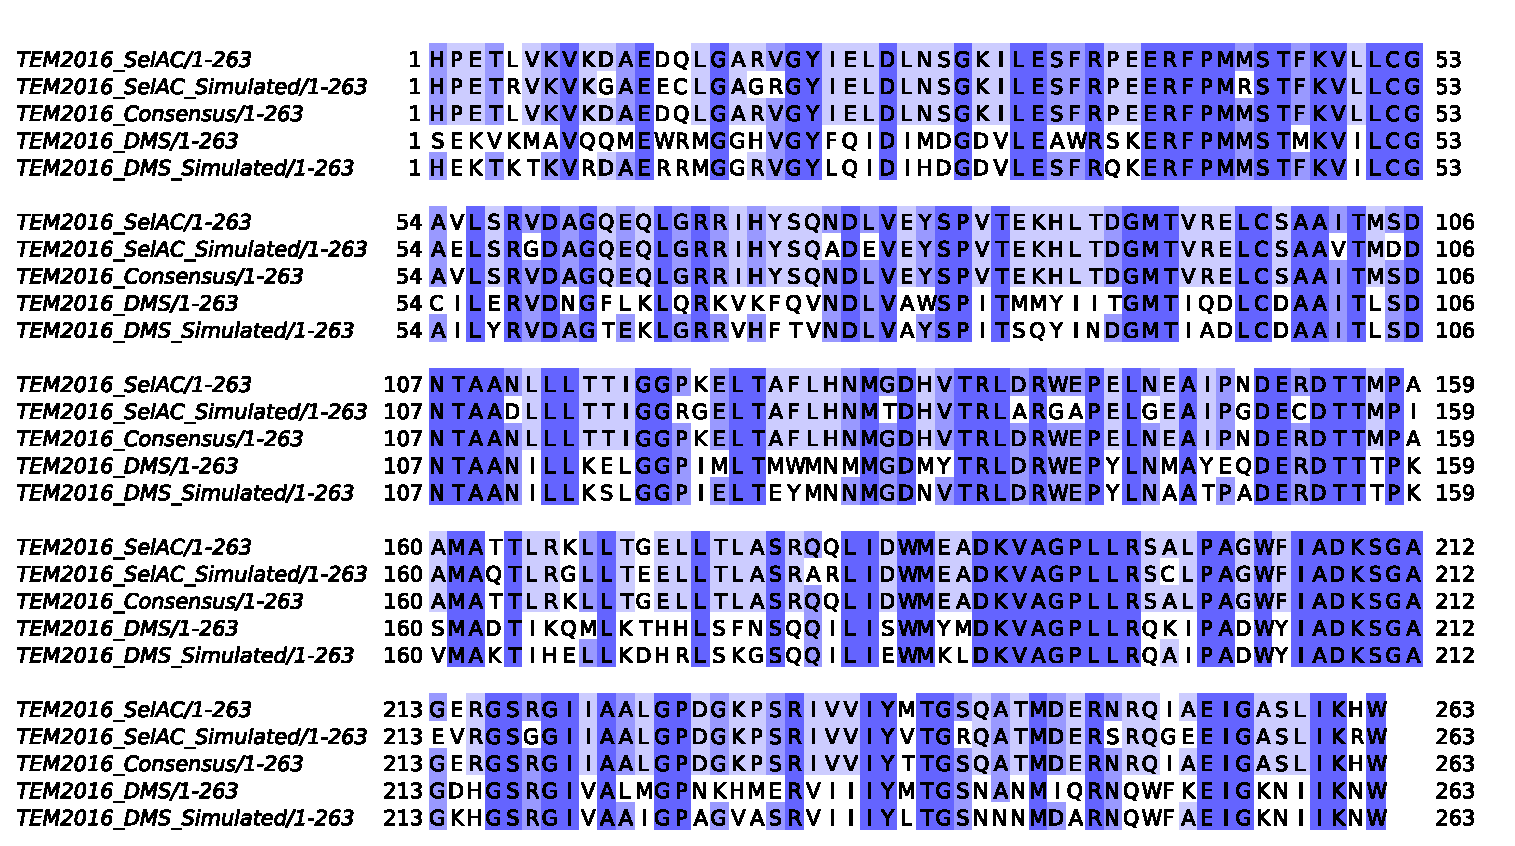
\includegraphics[width=\textwidth]{img/seq_simil_all.eps}
	\caption{Alignment of TEM optimal and simulated sequences. Indicated is the percentage identity at each site.}
	\label{fig:sim_seqs_cons}
\end{figure}

Simulations of codon sequences under the experimentally inferred site specific selection for amino acids reveals that we would not expect to see the observed TEM sequences.
We simulated under a wide range of effective population sizes $N_e$, and find that the experimentally inferred site specific selection is very strong.
With more realistic values of $N_e = 10^7$, we find that the simulated sequences are $62 \%$ similar to the observed consensus sequence (Figure \ref{fig:dms_sim}a).
This is a higher similarity than the observed consensus sequence shows with the sequence of selectively favored amino acids estimated using deep mutation scanning.
Only when $N_e$ is reduced to one individual does drift overpower selection (Figure \ref{fig:dms_sim}b).
The genetic load of the simulated sequences decrease slowly with increasing $N_e$ (Figure \ref{fig:dms_sim}b).
After simulating until the sequences reach one expected mutation per site and $N_e = 10^7$ the simulated sequences show a genetic load of 0.25, which is in contrast to the $\sim 8$ times higher than the estimated observed load of $2.1$.
Thus it appears unlikely that the observed sequences have evolved under the DMS inferred site specific selection values.


\begin{figure}[h]
    \centering
    \begin{subfigure}
        \centering
        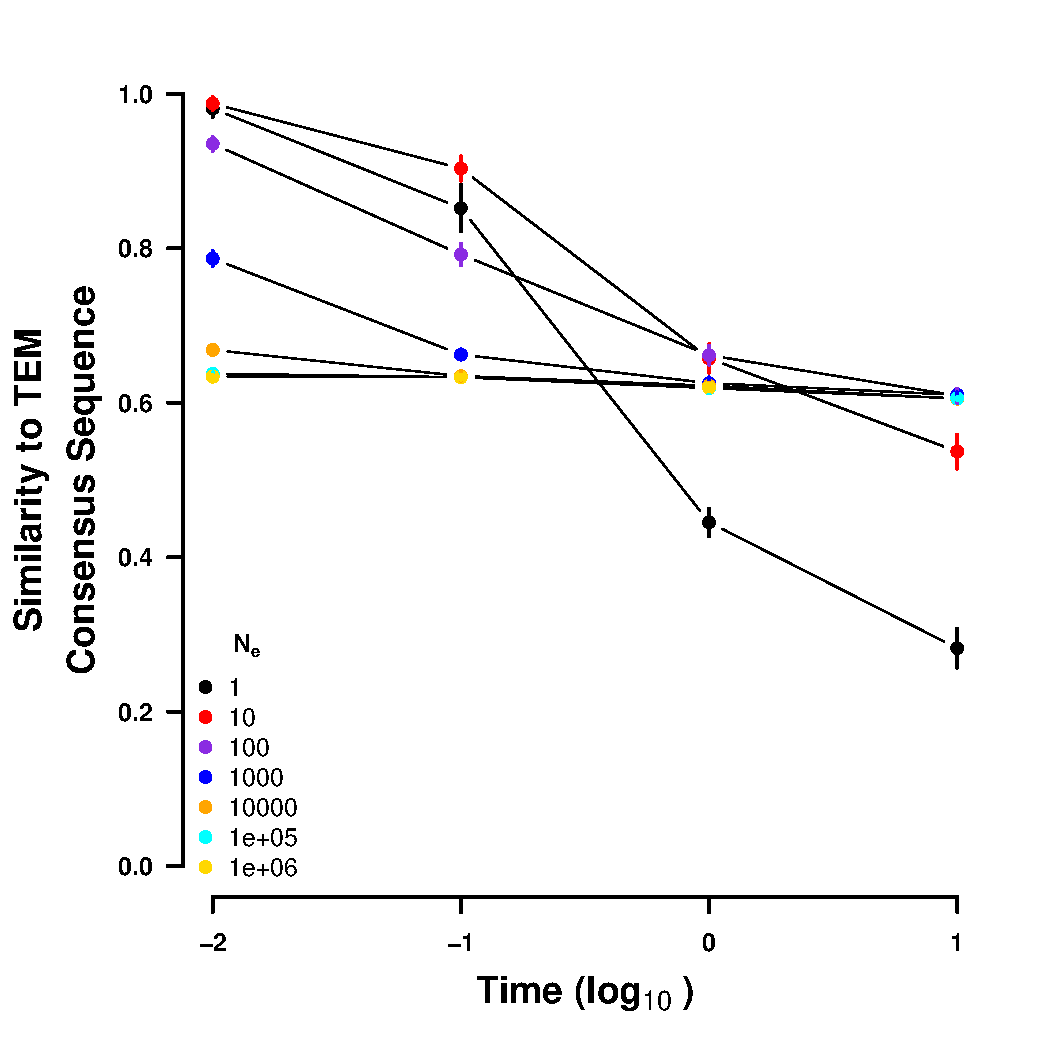
\includegraphics[width=.45\textwidth]{img/simulated_dist_time_DMS_ancest.pdf}
    \end{subfigure}
    \begin{subfigure}
        \centering
        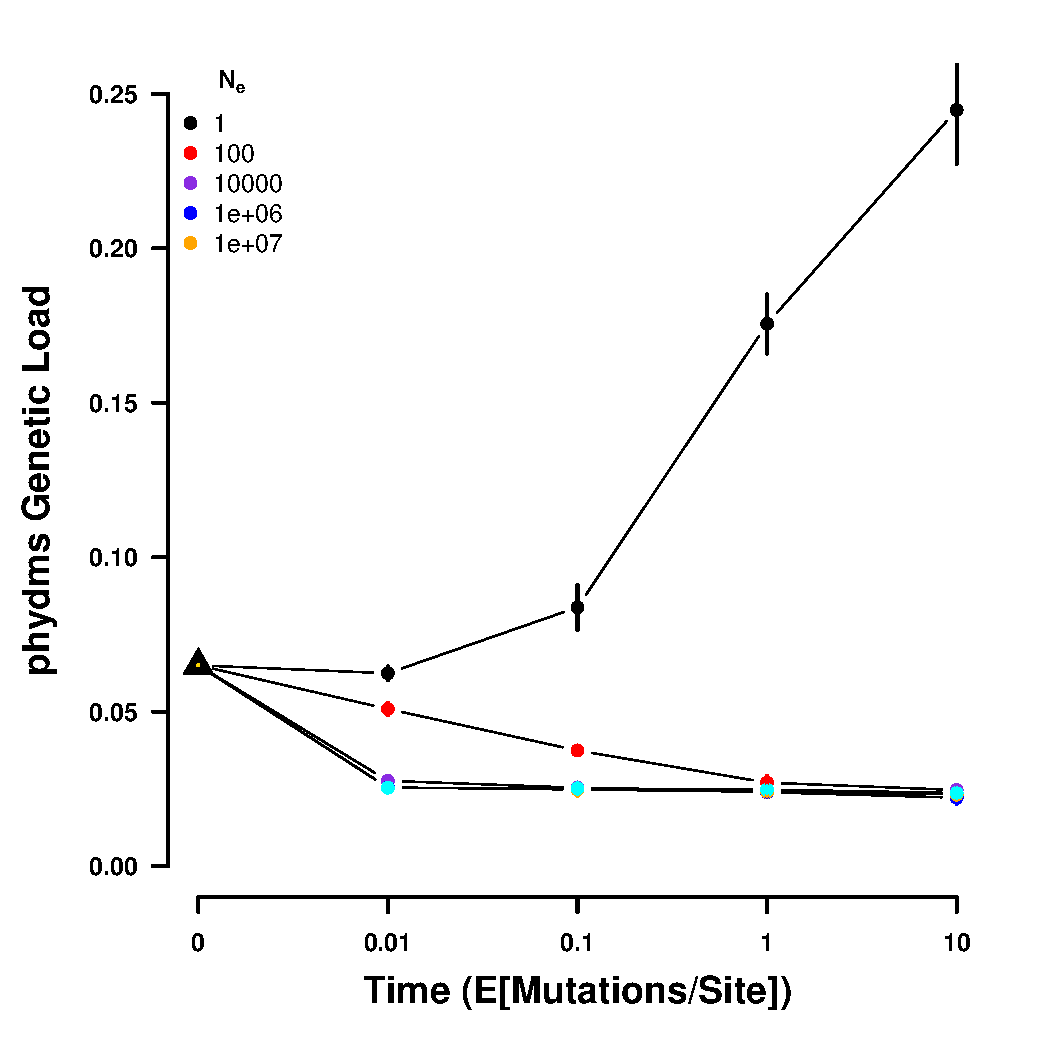
\includegraphics[width=.45\textwidth]{img/simulated_gl_time_DMS_ancest.pdf}
    \end{subfigure}
    \caption{Sequences simulated from the ancestral state under the site specific selection on amino acids estimated using deep mutation scanning. 
    (left) Sequence similarity to the observed consensus sequence at various times for a range on values of $N_e$.
    (right) Genetic load of the simulated sequences at various times for a range on values of $N_e$.
    Time is given in number of expected mutations per site, which equals the substitution rate of a neutral mutation.
    Points indicate sample means and vertical bars indicate standard deviations. Initial sequence is the inferred ancestral state of the TEM variants and indicated by a black triangle.}
    \label{fig:dms_sim}
\end{figure}

\subsection*{Stabilizing Selection for Optimal Physicochemical Properties Improves Model Adequacy} 
We assessed model adequacy of \selac and find that \selac better explains the observed TEM sequences.
The observed consensus sequence has $99 \%$ sequence similarity with the sequence of selectively favored amino acids estimated by \selac.
Furthermore, assuming the site specific selection estimated by \selac, the observed sequences represent a very small genetic load on the order of $10^{-6}$(Table \ref{tab:selection}, Figure \ref{fig:tem2016_sse}).

We simulated codon sequences forward in time for various length of time, using the \selac inferred site specific selection for amino acids to assess sequence similarity.
% Ancestral starting point
We simulated the evolution of TEM from the inferred ancestral state using a wide range of effective population sizes $N_e$ (Figure \ref{fig:selac_sim}a).
The ancestral state was estimated to be the observed consensus sequence.
As expected, for small $N_e$, simulated sequences drift away from the observed consensus sequence. 
Because of the high similarity between the optimal amino acid sequence estimated by \selac and the observed consensus sequence, the genetic load increases drastically as a result.
Increasing $N_e$ to $10^7$ the simulated sequences reach a sequence similarity of $83 \%$, this is in contrast to the observed avergage sequence similarity of $98 \%$.

We estimated the total genetic load the sequences represent using the \selac inferred selection on amino acids.
The total genetic load of the simulated sequences avergages $9.8\times10^{-6}$ (Figure \ref{fig:selac_sim}b).
The total estimated genetic load of the observed sequences averages $4.2\times 10^{-5}$.
Thus, the simulated sequences show a lower genetic load despite the greater divergence from the observed consensus sequence.

\begin{figure}[h]
    \centering
    \begin{subfigure}
        \centering
        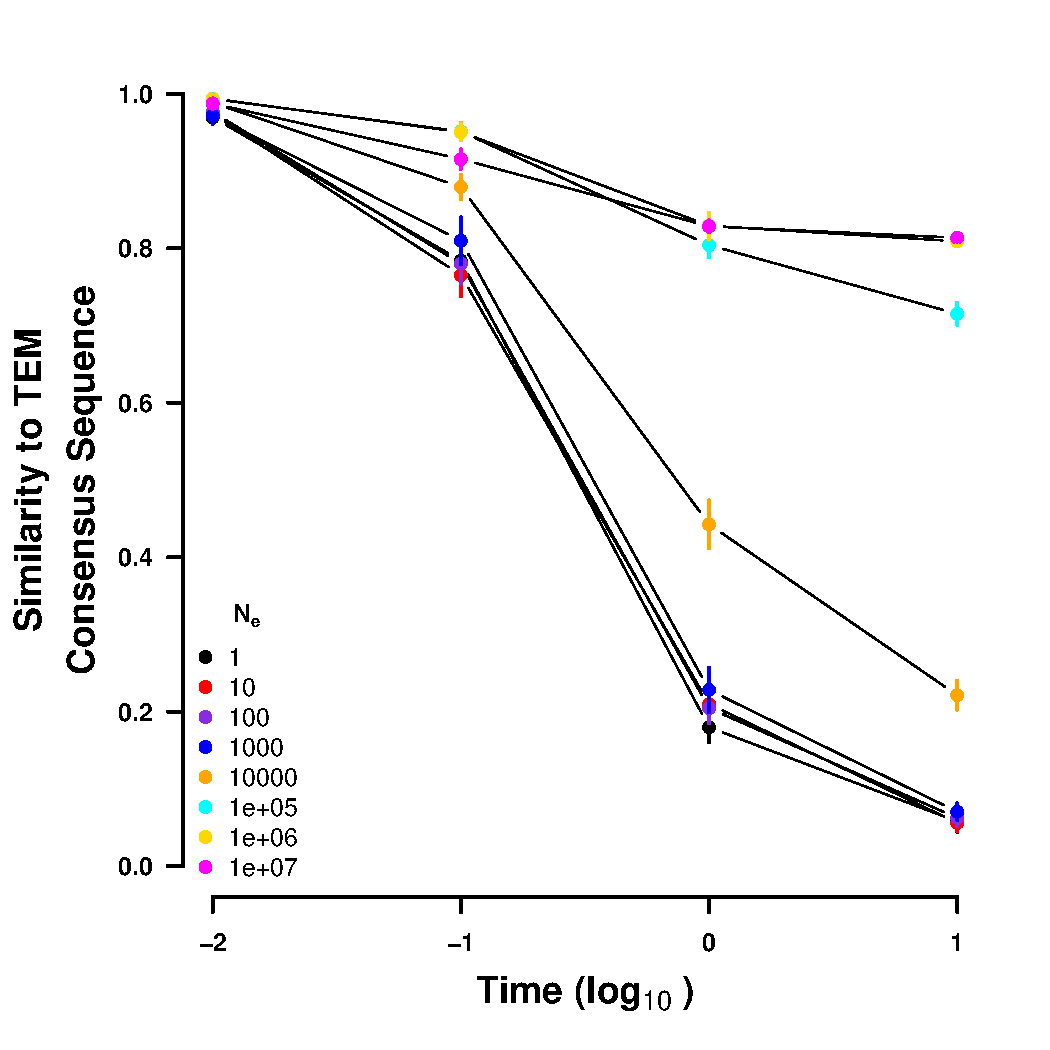
\includegraphics[width=.45\textwidth]{img/simulated_dist_time_SELAC_ancest.pdf}
    \end{subfigure}
    \begin{subfigure}
        \centering
        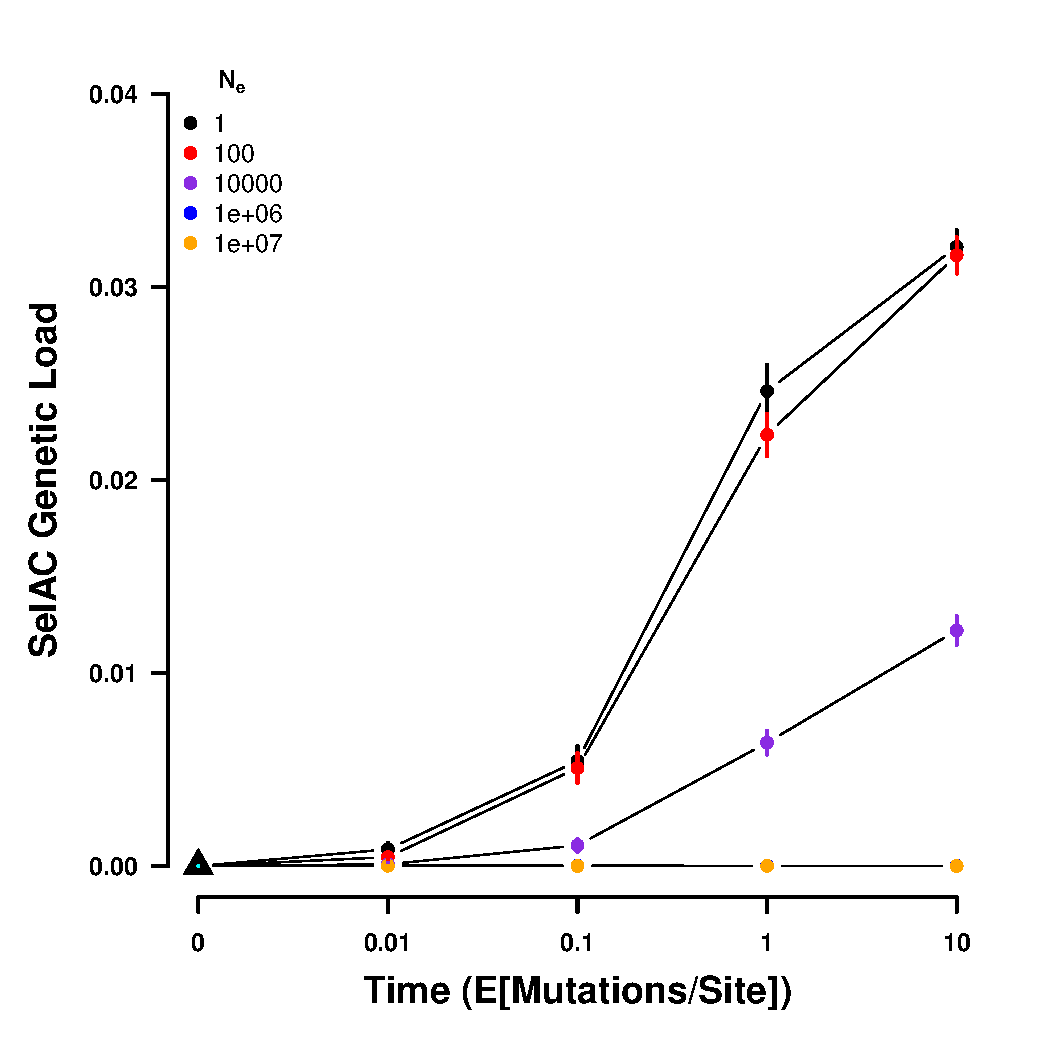
\includegraphics[width=.45\textwidth]{img/simulated_gl_time_SELAC_ancest.pdf}
    \end{subfigure}
    \caption{Sequences simulated from the ancestral state under the site specific selection on amino acids estimated using \selac. 
    (left) Sequence similarity to the observed consensus sequence at various times for a range on values of $N_e$.
    (right) Genetic load of the simulated sequences at various times for a range on values of $N_e$.
    Time is given in number of expected mutations per site, which equals the substitution rate of a neutral mutation.
    Points indicate sample means and vertical bars indicate standard deviations. Initial sequence is the inferred ancestral state of the TEM variants and indicated by a black triangle.}
    \label{fig:selac_sim}
\end{figure}

% Random starting point
To further demonstrate the consistency of \selac, we simulated codon sequences over the same period of time using $10$ uniform samples codon sequences with $263$ sites, the same length as the observed TEM variants.
We find that the sequence similarity increases with effective population size $N_e$.
The random sequences start of with a similarity of $\sim6 \%$ which increases with $N_e$ to $\sim28 \%$ (Figure \ref{fig:selac_sim_rand}a).
The same initial sequences under the site specific selection inferred by the deep mutation scanning experiment increase only to $\sim18 \%$ in sequence similarity.



\subsection*{Site Specific estimates of Selection on Amino Acids}
\selac allows for the estimation of site specific selection on amino acids and the genetic load of an observed amino acid relative to the inferred optimal amino acid.
Figure \ref{fig:tem2016_sse} and Figure \ref{fig:tem2016_3d} illustrate how the genetic load varies along the TEM sequence.
The region between residue $80$ to $120$ where three consecutive helices are located consist only of selectively favored amino acids and does not show any genetic load. 
The highest genetic load is found in the unstructured regions and the lowest genetic load is found in $\beta$-sheets.
Despite the differences, none show statistical significance.
The largest increase in genetic load is located at the beginning of the last helix.
This stronly contributes to the estimate of similar genetic loads for helices and unstructured regions in the observed TEM sequences (Table \ref{tab:selection}).
However, exclution of this site as outlier does not produce a significant difference in genetic load between unstructured and helix regions.

The highest efficacy of selection $G$ and the lowest genetic load among the TEM secondary structure features is estimated in the $\beta$-sheet regions.
Residues forming the active site appear to be under the strongest selection, with no accumulated genetic load (Table \ref{tab:selection}).
This is in concordance with the experimental estimates.
Again, differences between secondary structure elements are not statistically significant.

\begin{table}
  \centering
  \begin{tabular}{llrrrrr}
    & & & \multicolumn{2}{c}{G} & \multicolumn{2}{c}{Genetic Load} \\ 
    Protein & Secondary Structure & \# Residues	& \multicolumn{1}{c}{Mean} & \multicolumn{1}{c}{SE} & \multicolumn{1}{c}{Mean} & \multicolumn{1}{c}{SE} \\ \hline 
    TEM	&		& 263 & 219.3 & 7.5  & $15.9\times10^{-8}$ & $6.5\times10^{-8}$ \\
    &Helix 		& 113 & 206.1 & 12.4 & $17.5\times10^{-8}$ & $13.1\times10^{-8}$ \\
    &$\beta$-Sheet 	&  48 & 238.6 & 15.8 & $ 6.8\times10^{-8}$ & $2.9\times10^{-8}$ \\
    &Unstructured 	& 102 & 224.8 & 11.4 & $18.6\times10^{-8}$ & $8.1\times10^{-8}$ \\
    &Active Sites 	&   3 & 300   & 0    & 0      & 0      \\ \hline
    
    SHV&		& 263 & 244.9 & 6.8  & $4.0\times10^{-8}$ & $1.9\times10^{-8}$ \\
    &Helix		& 102 & 234.6 & 11.5 & $7.3\times10^{-8}$ & $4.8\times10^{-8}$ \\
    &$\beta$-Sheet 	&  66 & 253.1 & 12.8 & $2.1\times10^{-8}$ & $1.1\times10^{-8}$ \\
    &Unstructured	&  95 & 250.3 & 11.0 & $1.8\times10^{-8}$ & $0.6\times10^{-8}$  \\
    &Active Sites	&   3 & 199.9 & 100  & $2.4\times10^{-8}$ & $2.4\times10^{-8}$ \\

  \end{tabular}
  \caption{Efficacy of selection (G) and Genetic Load for TEM and SHV, and separated by secondary structure. G was estimated as a truncated variable with an upper bound of 300.}
  \label{tab:selection}
\end{table}

It was previously proposed that experimentally inferred site specific selection for amino acids can be used to extrapolate the fitness landscape of related proteins \citep{bloom2014, bloom2017}.
We therefore compared the genetic load, the \selac selection parameters of our \selac TEM model fit to a \selac model fit of SHV, and site specific efficacy of selection ($G$).
The genetic load in SHV appears to be lower than in TEM with the exception of residues found in $\beta$-sheets and the active site (Table \ref{tab:selection}).
This is consistent with the elevated efficacy of selection $G$ in SHV.
However, only differences in genetic load in the unstructured regions are significantly different between the TEM and SHV sequences, but only at the $\alpha = 0.05$ significant level ($p = 0.04$).
While the average genetic load across secondary structures is not significantly different, the sites causing increases genetic load differ between SHV and TEM (Figure \ref{fig:shv2016_sse}).
In contrast to TEM, we find the highest genetic load in SHV secondary structure features in the helices (Table \ref{tab:selection}).
We find the highest genetic load in SHV at the end of the first helix.
However, we do find a peak of similar magnitude in the TEM sequence at the end of the first helix, but this peak is overshadowed by increased genetic load at the beginning of the last helix.

We find that site specific efficacy of selection $G$ differs greatly between SHV and TEM ($\rho = 0.12$), despite a similar estimate of $\alpha_G$ describing the distribution of $G$ values (Figure \ref{fig:tem_shv_param_comp}a).
We generally find increased G values in SHV, with the exception of the active site (Table \ref{tab:selection}).
However, non of these increases are statistically significant.
Most \selac selection parameters are very similar between the TEM and the SHV model fit. 
An exception is the weight for the \PC composition property $\alpha_c$ (Figure \ref{fig:tem_shv_param_comp}b).
Furthermore, we find that the sequences of selectively favored amino acids estimated by \selac for TEM and SHV only show $68 \%$ sequence similarity.



\begin{figure}[H]
     \centering
	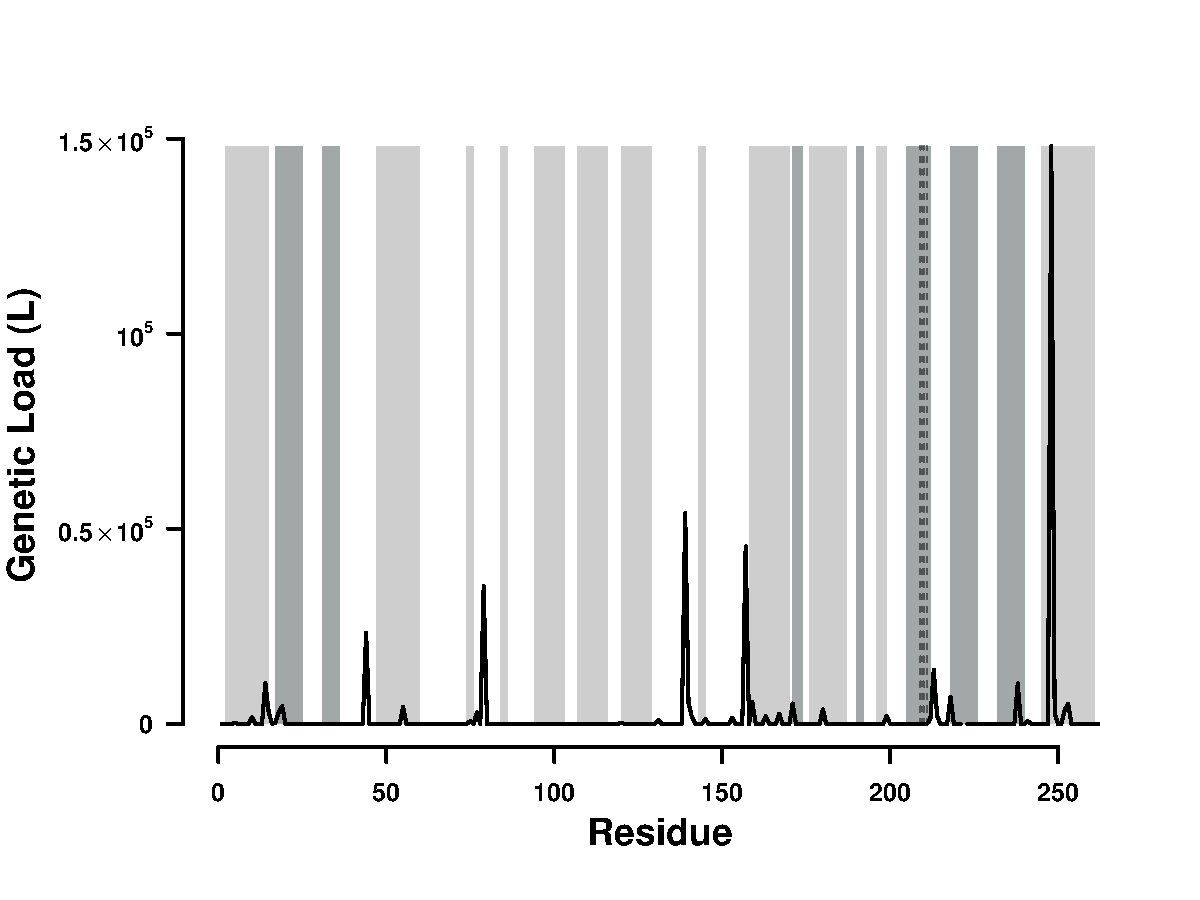
\includegraphics[width=\textwidth]{img/GL_slide_TEM2016}
	\caption{Distribution of genetic load in TEM. 
	Average genetic load over all observed TEM variants is indicated by the black line. 
	Light gray bars indicate where helices are found, and dark gray bars indicate $\beta$-sheets.
	The three residues forming the active sites are indicated by three triangles at the top of the plot.}
	\label{fig:tem2016_sse}
\end{figure}

\section*{Discussion}

Here we revisited how well experimental selection estimates from laboratory experiments, specifically deep mutation scanning, explain sequence evolution and compared it to \selac, a novel phylogenetic framework.
Previous work has shown that laboratory estimates of selection can improve model fit over classical approaches like GY94 \citep{bloom2014, bloom2017}.
While our study confirms this notion, we identify important shortcomings of these laboratory estimates.
In contrast, \selac is a more general phylogenetic model of stabilizing selection that does not require costly laboratory estimates of selection and is nevertheless favored by model selection (Table \ref{tab:AIC}).
\selac does not rely on artificially induced selection in the laboratory but is a mechanistic framework rooted in first principles.
It estimates site specific selection on amino acids from the sequence data based on distances between amino acids in \PC space \citep{grantham1974,beaulieu2018}.
This allows \selac to be applied to any set of protein coding sequences, eliminating the need to extrapolate from one homologous gene family to the next (e.g. from TEM to SHV).

While previous work showed the advantages of experimentally informed phylogenetics, they did not assess how adequate the estimated selection reflects observed wild-type sequences.
The low sequence similarity between the observed consensus sequence and the sequence of selectively favored amino acids estimated from deep mutation scanning experiments is evidence for that.
This begs the question how well the experimental selection coefficients represent evolution of sequences in nature.
Deep mutation scanning experiments are performed using a comprehensive library of mutants and a strong artificial selection pressure \citep{FirnbergAndOstermeier2012, Jain2014, FowlerAndFields2014, Fowler2014}.
This results in a very large selection coefficient $s$ and a heterogeneous population of competing individuals unlikey to occur in nature.

The selection pressure imposed during the DMS experiment was limited to ampicillin and focused solely on TEM-1 \citep{stiffler2016}.
However, TEM variants can also confer resistance to a wide range of other antibiotics, including penicillins, cephalosporins, cefotaxime, ceftazidime, or aztreonam \citep{sougakoff1988,sougakoff1989,goussard1991,mabilat1992,chanal1992,brun1994}.
Thus, the inferred selection is biased towards ampicillin and is inconsistent with the observed TEM sequences (Figure \ref{fig:dms_sim}).
This may very well be very appropriate to explore the selection on TEM in a hospital environment but is unlikely to be representative of the selection faced by \ecoli in nature.
%We therefore propose to include a variety of selection pressures if the experimental selection estimates are used for phylogenetic inference.

%TODO:  Lack of repeatability between labs introduces further problems (Firnberg et al 2014 vs. Stifler et al. 2016).

If we assume that the DMS selection coefficients underly the evolution of the observed TEM sequences we are left with two possible explanations for the observed sequences.
First, the sequences are unable to reach a fitness peak, potentially due to a low selection pressure, or not enough time.
Second, the observed TEM sequences are highly maladapted.
Both options seem unlikely.
\ecoli has a large effective population size $N_e$, estimates are on the order of $10^8$ to $10^9$ \citep{OchmanAndWilson1987, hartl1994}.
As new mutations are introduced into a population at a rate proportional to $N_e$, \ecoli can effectively explore the sequence space.
However, this also raises concerns that the population mutation rate of \ecoli $\Theta = 4N_e\mu$ exceeds $0.1$ and violated \selac's weak mutation assumption \citep{deKoning259507}.
We therefore expect the observed sequence variants to be near mutation-selection-drift equilibrium.
This expectation is supported by our simulations in which we observe a higher sequence similarity with the observed TEM consensus sequence and decreased genetic load even with much smaller $N_e$ (Figure \ref{fig:dms_sim}).
Furthermore, previous work showed that the catalytic reaction performed by TEM of penicillin-class antibiotics is close the diffusion limit, making TEM a so-called perfect enzyme \citep{matagne1998}.

As experimental selection estimates are not readily available for most organsims and proteins, one solution is to extrapolate the estimates to homologous gene families \citep{bloom2014, bloom2017}.
When extrapolating the selection estimates from the $\beta$-lactamase family TEM to the SHV family, the sequence similarity between the observed consensus sequence and the sequence of selectively favored amino acids estimated from deep mutation scanning experiments drops slightly from $52 \% $ to $49 \%$.
In contrast, the site specific efficacy of selection (G) revealed large differences in the site specific selection on amino acids between TEM and SHV.
The mismatched in \PC weights also indicates differences in selection constraints. 
While the polarity of amino acids is of similar importance in TEM and SHV, amino acid composition plays a much greater role in SHV than in TEM.
In contrast to the experimental selection estimates, the \selac selection estimates are consistent with the observed sequences, e.g. the selectively favored amino acids estimated by \selac shows a high sequence similarity with the observed TEM and SHV consensus sequence ($99 \%$).

While \selac better explains the observed TEM sequences than the experimental estimates of site specific selection on amino acids, it is not without shortcomings itself.
\selac is currently to slow to be used in topology searches, therefore it is unclear if the differences in topology between \phydms and \selac can be attributed to the same inadequacies of experimentally inferred selection.
As the simulation of TEM evolution from he ancestral state under the \selac inferred site specific selection revealed, the formulation of \selac can and should be improved upon.
Starting from the ancestral sequence, the simulated sequences show initial divergence despite stabilizing selection for the optimal amino acid.
While \selac allows for site heterogeneity in selection for amino acids, it still ignores epistatis.
This however, is a shortcoming shared with experimental estimates by deep mutation scanning, as each mutant typically only carries one mutation \citep{FirnbergAndOstermeier2012, Jain2014}.
\selac is a model stabilizing selection, however, not every protein is under stabilizing selection.
TEM plays a role in chemical warfare with conspecifics and other microbes, therefore some sites may be under negative frequency dependent selection.
This potential heterogeneity in selection highlights another shortcoming of \selac.
\selac assumes the same distribution for the efficacy of selection (G) and \PC sensitivities across the whole protein.
However, it is easy to imagine that sites in different secondary structures or at active sites do not share a common distribution.

% TODO: talk about that random sequences still have 30% functionallity under selac. Could explain why the  simulation from the ancestral state diverges to ~80 %. Or maybe do we underestimate selection?

As \selac assumes that the fitness of an amino acid at a site declines with its distance in \PC space to the optimal amino acid, the choice of \PC properties becomes important.
In this study, we assumed the \PC properties estimated by \citet{grantham1974} for all sites.
However, a wide range of additional \PC properties of amino acids have been described \citep{Kawashima2008}.
A more optimal choice of \PC properties may be possible as well as the a relaxation of the assumptions that the same properties apply to all sites equally.
Future work will attempt to address these shortcomings, however, \selac's hierarchical model structure and the open-source code base allow researchers to easily address these shortcoming if desired.

In conclusion, experimental estimates of site specific selection on amino acids have to be treated with skepticism and their adequacy should be assessed before using them to inform phylogenetic inferences.
This study was initiated to assess the quality of \selac with the expectation that \selac could be a faster, cheaper, and more readily available alternative to experimentally inferred selection;
specifically in organisms where these experiments are not feasible.
Intuitively one would expect that selection coefficients estimated of mutations in living organisms would provide more information on the evolution of proteins than a model relying on many simplifying assumptions.
As we show in this study, not only can \selac estimate site specific selection on amino acids but our approach is a more adequat descripton of selection on amino acids in nature than experimental estimates.


\section*{Materials and Methods}

\subsection*{Phylogenetic Inference and Model selection}

TEM and SHV sequences were obtained from \citet{bloom2017} already aligned.
We however, separated the TEM and SHV sequences into individual alignments.
Experimentally fitness values for TEM were taken from \citet{stiffler2016}.
We followed \citep{bloom2017} to convert the experimental fitness values into site specific equilibrium frequencies for \phydms. 
\phydms (version 2.5.1) was fitted using site specific selection on amino acids estimated from deep mutation scanning experiments from \citet{stiffler2016} and python (version 3.6).

\selac (version 1.6.1) was fitted to the TEM alignment using R (version 3.4.1) \citep{rcore} with and without site specific selection on amino acids estimated from deep mutation scanning experiments.
We assumed the \PC properties estimated by \citet{grantham1974}.
We chose the contraint free  general unrestricted model \citep{yang1994} as mutation model .
All other models were fitted using IQTree \citep{nguyen2015}.

We report each model's $\log(\Lik)$, AIC, and  AICc. 
Models were selected based on the AICc values.

\subsection*{Sequence Simulation}

Sequences were simulated by stochastic simulations using a Gillespie algorithm \citep{gillespie1976} that was model independent.
The simulation followed \citet{SellaAndHirsh2005} to calculate fixation probabilities.
The fitness values were estimated using \selac or experimentally inferred.
We chose the fitness values of the highest concentration (2500 $\mu g/mL$) treatment of ampicillin for our comparison.
We modified the experimental fitness such that the amino acid with the highest fitness at each site has a value of one.
Mutation rates were taken from the \selac or \selacDMS fit.
The initial sequences were either a random sample of 263 codons or the ancestral sequence reconstructed using FastML \citep{fastml} (last accessed: 30.09.2018).
Each sequence was simulated 10 times and we report average genetic load and sequence similarity and the corresponding standard error.
The sequences were sampled at times 0.01, 0.1, 1, and 10 expected mutations per site.

\subsection*{Estimating site specific efficacy of selection G}

\selac does not by default estimate site specific values for $G$ but assusmes G values follow a gamma distribution \citep{Felsenstein2001}.
Site specific values for $G$ were optimized by fixing all estimated parameters and perfoming a maximum likelihood search without the usual integration over $G$.
In contrast to \selac that assumes $G$ to be purley positive, we allowed negative values for $G$ and constraint the search to values between $-300$ and $300$.

\subsection*{Estimating site specific fitness values $w_i$}

Following \citet{beaulieu2018} $w_i$ is proportional to
\begin{equation}
w_i \propto \exp(-A_0\eta\psi)
\end{equation}
were $A_0$ describes the decline in fitness with each high energy phosphate bond wasted per unit time, and $\psi$ is the protein's production rate.
$\eta$ is the cost/benefit ratio of a protein (see \citep{beaulieu2018} for details). 
However, \selac only estimates a composition parameter $\psi' = A_0\psi N_e$.
$N_e$ describes the effective population size.
\selac assumes $N_e = 5\times 10^6$.
\selac assumes $A_0 = 4 \times 10{-7}$ \citep{gilchrist2007}.
Thus, 
\begin{equation}
\psi = \frac{\psi'}{A_0N_eq}
\end{equation}


\subsection*{Model Adequacy}

Model adequacy was assessed by comparing the observed sequences and simulations under the site specific selection inferred by the deep mutation scanning experiment or \selac.
First, similarity between the sequence of selectively favored amino acids and the observed TEM sequences was assessed.
Sequence similarity was measured as the number of differences in the amino acid sequence.
Second, the genetic load of the observed and the simulated sequences was calculated using either the site specific selection inferred by the deep mutation scanning experiment or \selac.

Genetic load was calculated as
\begin{equation}
L_i = \frac{w_{max} - w_i}{w_{max}}
\end{equation}
were $w_{max}$ is the fitness of the sequence of selectively favored amino acids estimated using  the site specific selection inferred by the deep mutation scanning experiment or \selac.
$w_i$ represents the fitness of the $i$th residue.
This the genetic load $L$ of a sequence is given by $\sum_{i=1}^n L_i$ where $n$ is the number of amino acids.

\section*{Acknowledgments}

This work was supported in part by NSF Award and DEB-1355033 (BCO, MAG, and RZ) with additional support from The University of Tennessee Knoxville. 
CL received support as a Graduate Student Fellow at the National Institute for Mathematical and Biological Synthesis, an Institute sponsored by the National Science Foundation through NSF Award DBI-1300426, with additional support from UTK. 
The authors would like to thank Russel Zaretzki, Jeremy Beaulieu and Alexander Cope for their helpful criticisms and suggestions for this work.




\bibliographystyle{plain}
\bibliography{ecoli}

\clearpage
\beginsupplement
\section*{Supplementary Material}

  \singlespacing
\singlespacing
\begin{longtable}{clrrrrrr}
	No. & Model & LnL & n & AIC & $\Delta$AIC & AICc & $\Delta$AICc \\ \hline
	1 & \selacDMS+G4 & -1768 & 111 & 3758 & 14 & 3760 & 0 \\ 
	2 & \selac+G4 & -1498 & 374 & 3744 & 0 & 3766 & 6 \\ 
	3 & \phydms & -2060.85 & 102 & 4326 & 582 & 4328 & 568 \\ 
	4 & SYM+R2 & -2229.616 & 102 & 4663.232 & 919.232 & 4693.862 & 933.862 \\ 
	5 & TIMe+R2 & -2232.406 & 100 & 4664.811 & 920.811 & 4694.172 & 934.172 \\ 
	6 & TVMe+R2 & -2232.838 & 101 & 4667.677 & 923.677 & 4697.668 & 937.668 \\ 
	7 & TIM3e+R2 & -2234.332 & 100 & 4668.664 & 924.664 & 4698.024 & 938.024 \\ 
	8 & TIM2e+R2 & -2234.381 & 100 & 4668.763 & 924.763 & 4698.123 & 938.123 \\ 
	9 & K3P+R2 & -2235.777 & 99 & 4669.553 & 925.553 & 4698.291 & 938.291 \\ 
	10 & TNe+R2 & -2236.078 & 99 & 4670.155 & 926.155 & 4698.892 & 938.892 \\ 
	11 & SYM+R3 & -2229.616 & 104 & 4667.232 & 923.232 & 4699.162 & 939.162 \\ 
	12 & TIM+F+R2 & -2230.958 & 103 & 4667.915 & 923.915 & 4699.191 & 939.191 \\ 
	13 & TIMe+R3 & -2232.404 & 102 & 4668.808 & 924.808 & 4699.437 & 939.437 \\ 
	14 & GTR+F+R2 & -2228.537 & 105 & 4667.073 & 923.073 & 4699.665 & 939.665 \\ 
	15 & K3Pu+F+R2 & -2232.617 & 102 & 4669.234 & 925.234 & 4699.864 & 939.864 \\ 
	16 & TVM+F+R2 & -2230.105 & 104 & 4668.21 & 924.21 & 4700.14 & 940.14 \\ 
	17 & TVMe+R3 & -2232.838 & 103 & 4671.676 & 927.676 & 4702.952 & 942.952 \\ 
	18 & K2P+R2 & -2239.424 & 98 & 4674.847 & 930.847 & 4702.969 & 942.969 \\ 
	19 & TIM3e+R3 & -2234.332 & 102 & 4672.664 & 928.664 & 4703.293 & 943.293 \\ 
	20 & TIM2e+R3 & -2234.381 & 102 & 4672.762 & 928.762 & 4703.391 & 943.391 \\ 
	21 & TIM3+F+R2 & -2233.064 & 103 & 4672.127 & 928.127 & 4703.403 & 943.403 \\ 
	22 & TIM2+F+R2 & -2233.114 & 103 & 4672.227 & 928.227 & 4703.503 & 943.503 \\ 
	23 & K3P+R3 & -2235.777 & 101 & 4673.553 & 929.553 & 4703.545 & 943.545 \\ 
	24 & TN+F+R2 & -2234.624 & 102 & 4673.249 & 929.249 & 4703.878 & 943.878 \\ 
	25 & TPM3u+F+R2 & -2234.673 & 102 & 4673.347 & 929.347 & 4703.977 & 943.977 \\ 
	26 & TPM3+F+R2 & -2234.674 & 102 & 4673.348 & 929.348 & 4703.978 & 943.978 \\ 
	27 & TPM2u+F+R2 & -2234.681 & 102 & 4673.363 & 929.363 & 4703.993 & 943.993 \\ 
	28 & TPM2+F+R2 & -2234.683 & 102 & 4673.365 & 929.365 & 4703.995 & 943.995 \\ 
	29 & TNe+R3 & -2236.077 & 101 & 4674.155 & 930.155 & 4704.146 & 944.146 \\ 
	30 & TIM+F+R3 & -2230.958 & 105 & 4671.915 & 927.915 & 4704.507 & 944.507 \\ 
	31 & HKY+F+R2 & -2236.266 & 101 & 4674.531 & 930.531 & 4704.522 & 944.522 \\ 
	32 & GTR+F+R3 & -2228.536 & 107 & 4671.073 & 927.073 & 4705.011 & 945.011 \\ 
	33 & K3Pu+F+R3 & -2232.617 & 104 & 4673.234 & 929.234 & 4705.163 & 945.163 \\ 
	34 & TVM+F+R3 & -2230.105 & 106 & 4672.21 & 928.21 & 4705.471 & 945.471 \\ 
	35 & K2P+R3 & -2239.192 & 100 & 4678.384 & 934.384 & 4707.745 & 947.745 \\ 
	36 & TIM3+F+R3 & -2233.063 & 105 & 4676.127 & 932.127 & 4708.718 & 948.718 \\ 
	37 & TIM2+F+R3 & -2233.113 & 105 & 4676.227 & 932.227 & 4708.818 & 948.818 \\ 
	38 & TN+F+R3 & -2234.624 & 104 & 4677.249 & 933.249 & 4709.178 & 949.178 \\ 
	39 & TPM3u+F+R3 & -2234.673 & 104 & 4677.347 & 933.347 & 4709.277 & 949.277 \\ 
	40 & TPM3+F+R3 & -2234.674 & 104 & 4677.348 & 933.348 & 4709.277 & 949.277 \\ 
	41 & TPM2u+F+R3 & -2234.681 & 104 & 4677.363 & 933.363 & 4709.293 & 949.293 \\ 
	42 & TPM2+F+R3 & -2234.682 & 104 & 4677.364 & 933.364 & 4709.294 & 949.294 \\ 
	43 & HKY+F+R3 & -2236.074 & 103 & 4678.148 & 934.148 & 4709.424 & 949.424 \\ 
	44 & SYM+I+G4 & -2243.212 & 102 & 4690.424 & 946.424 & 4721.054 & 961.054 \\ 
	45 & TVMe+I+G4 & -2244.533 & 101 & 4691.066 & 947.066 & 4721.057 & 961.057 \\ 
	46 & TIMe+I+G4 & -2246.457 & 100 & 4692.914 & 948.914 & 4722.275 & 962.275 \\ 
	47 & K3P+I+G4 & -2248.166 & 99 & 4694.332 & 950.332 & 4723.069 & 963.069 \\ 
	48 & TVM+F+I+G4 & -2241.853 & 104 & 4691.707 & 947.707 & 4723.636 & 963.636 \\ 
	49 & TIM3e+I+G4 & -2247.379 & 100 & 4694.758 & 950.758 & 4724.119 & 964.119 \\ 
	50 & K3Pu+F+I+G4 & -2245.156 & 102 & 4694.311 & 950.311 & 4724.941 & 964.941 \\ 
	51 & GTR+F+I+G4 & -2241.484 & 105 & 4692.968 & 948.968 & 4725.559 & 965.559 \\ 
	52 & TIM+F+I+G4 & -2244.418 & 103 & 4694.836 & 950.836 & 4726.112 & 966.112 \\ 
	53 & TPM3u+F+I+G4 & -2246.03 & 102 & 4696.06 & 952.06 & 4726.69 & 966.69 \\ 
	54 & TPM3+F+I+G4 & -2246.069 & 102 & 4696.138 & 952.138 & 4726.768 & 966.768 \\ 
	55 & TIM2e+I+G4 & -2248.934 & 100 & 4697.868 & 953.868 & 4727.228 & 967.228 \\ 
	56 & TNe+I+G4 & -2250.587 & 99 & 4699.174 & 955.174 & 4727.911 & 967.911 \\ 
	57 & TIM3+F+I+G4 & -2245.534 & 103 & 4697.068 & 953.068 & 4728.344 & 968.344 \\ 
	58 & K2P+I+G4 & -2252.181 & 98 & 4700.362 & 956.362 & 4728.484 & 968.484 \\ 
	59 & TPM2u+F+I+G4 & -2247.579 & 102 & 4699.158 & 955.158 & 4729.788 & 969.788 \\ 
	60 & TPM2+F+I+G4 & -2247.685 & 102 & 4699.371 & 955.371 & 4730 & 970 \\ 
	61 & HKY+F+I+G4 & -2249.065 & 101 & 4700.13 & 956.13 & 4730.121 & 970.121 \\ 
	62 & TIM2+F+I+G4 & -2247.009 & 103 & 4700.018 & 956.018 & 4731.294 & 971.294 \\ 
	63 & TN+F+I+G4 & -2248.511 & 102 & 4701.023 & 957.023 & 4731.652 & 971.652 \\ 
	64 & TVMe+I & -2254.804 & 100 & 4709.608 & 965.608 & 4738.968 & 978.968 \\ 
	65 & K3P+I & -2257.72 & 98 & 4711.439 & 967.439 & 4739.561 & 979.561 \\ 
	66 & SYM+I & -2254.11 & 101 & 4710.221 & 966.220 & 4740.212 & 980.212 \\ 
	67 & TIMe+I & -2257.074 & 99 & 4712.149 & 968.149 & 4740.886 & 980.886 \\ 
	68 & TVM+F+I & -2252.157 & 103 & 4710.315 & 966.315 & 4741.591 & 981.591 \\ 
	69 & K3Pu+F+I & -2254.856 & 101 & 4711.712 & 967.712 & 4741.704 & 981.704 \\ 
	70 & TIM3e+I & -2257.796 & 99 & 4713.592 & 969.592 & 4742.33 & 982.33 \\ 
	71 & TPM3+F+I & -2255.771 & 101 & 4713.543 & 969.543 & 4743.534 & 983.534 \\ 
	72 & TPM3u+F+I & -2255.771 & 101 & 4713.543 & 969.543 & 4743.534 & 983.534 \\ 
	73 & K2P+I & -2261.218 & 97 & 4716.436 & 972.436 & 4743.949 & 983.949 \\ 
	74 & GTR+F+I & -2252.067 & 104 & 4712.133 & 968.133 & 4744.063 & 984.063 \\ 
	75 & TIM+F+I & -2254.783 & 102 & 4713.566 & 969.566 & 4744.195 & 984.195 \\ 
	76 & TNe+I & -2260.579 & 98 & 4717.158 & 973.158 & 4745.28 & 985.28 \\ 
	77 & TIM3+F+I & -2255.684 & 102 & 4715.368 & 971.368 & 4745.998 & 985.998 \\ 
	78 & HKY+F+I & -2258.352 & 100 & 4716.703 & 972.703 & 4746.064 & 986.064 \\ 
	79 & TIM2e+I & -2259.878 & 99 & 4717.757 & 973.757 & 4746.494 & 986.494 \\ 
	80 & TVMe+G4 & -2258.853 & 100 & 4717.705 & 973.705 & 4747.066 & 987.066 \\ 
	81 & SYM+G4 & -2257.573 & 101 & 4717.146 & 973.146 & 4747.137 & 987.137 \\ 
	82 & TPM2+F+I & -2257.712 & 101 & 4717.423 & 973.423 & 4747.415 & 987.415 \\ 
	83 & TPM2u+F+I & -2257.712 & 101 & 4717.423 & 973.423 & 4747.415 & 987.415 \\ 
	84 & K3P+G4 & -2261.922 & 98 & 4719.844 & 975.844 & 4747.966 & 987.966 \\ 
	85 & TIMe+G4 & -2260.683 & 99 & 4719.365 & 975.365 & 4748.103 & 988.103 \\ 
	86 & TN+F+I & -2258.28 & 101 & 4718.561 & 974.561 & 4748.552 & 988.552 \\ 
	87 & TIM3e+G4 & -2261.255 & 99 & 4720.51 & 976.51 & 4749.247 & 989.247 \\ 
	88 & TVM+F+G4 & -2256.108 & 103 & 4718.216 & 974.216 & 4749.492 & 989.492 \\ 
	89 & TIM2+F+I & -2257.643 & 102 & 4719.286 & 975.286 & 4749.915 & 989.915 \\ 
	90 & K3Pu+F+G4 & -2258.971 & 101 & 4719.941 & 975.941 & 4749.933 & 989.933 \\ 
	91 & TPM3u+F+G4 & -2259.716 & 101 & 4721.433 & 977.433 & 4751.424 & 991.424 \\ 
	92 & TPM3+F+G4 & -2259.717 & 101 & 4721.434 & 977.434 & 4751.425 & 991.425 \\ 
	93 & GTR+F+G4 & -2255.75 & 104 & 4719.5 & 975.5 & 4751.43 & 991.43 \\ 
	94 & TIM+F+G4 & -2258.638 & 102 & 4721.276 & 977.276 & 4751.906 & 991.906 \\ 
	95 & K2P+G4 & -2265.454 & 97 & 4724.907 & 980.907 & 4752.421 & 992.421 \\ 
	96 & TNe+G4 & -2264.219 & 98 & 4724.437 & 980.437 & 4752.559 & 992.559 \\ 
	97 & TIM3+F+G4 & -2259.366 & 102 & 4722.732 & 978.732 & 4753.361 & 993.361 \\ 
	98 & TIM2e+G4 & -2263.57 & 99 & 4725.141 & 981.141 & 4753.878 & 993.878 \\ 
	99 & JC+R2 & -2266.233 & 97 & 4726.466 & 982.466 & 4753.98 & 993.98 \\ 
	100 & F81+F+R2 & -2262.327 & 100 & 4724.654 & 980.654 & 4754.015 & 994.015 \\ 
	101 & HKY+F+G4 & -2262.499 & 100 & 4724.999 & 980.999 & 4754.359 & 994.359 \\ 
	102 & TPM2+F+G4 & -2261.915 & 101 & 4725.829 & 981.829 & 4755.82 & 995.82 \\ 
	103 & TPM2u+F+G4 & -2261.915 & 101 & 4725.829 & 981.829 & 4755.82 & 995.82 \\ 
	104 & TN+F+G4 & -2262.169 & 101 & 4726.338 & 982.338 & 4756.329 & 996.329 \\ 
	105 & TIM2+F+G4 & -2261.585 & 102 & 4727.17 & 983.17 & 4757.8 & 997.8 \\ 
	106 & F81+F+R3 & -2262.028 & 102 & 4728.056 & 984.056 & 4758.685 & 998.685 \\ 
	107 & JC+R3 & -2265.997 & 99 & 4729.994 & 985.994 & 4758.731 & 998.731 \\ 
	108 & F81+F+I+G4 & -2274.845 & 100 & 4749.69 & 1005.69 & 4779.05 & 1019.05 \\ 
	109 & JC+I+G4 & -2279.318 & 97 & 4752.636 & 1008.636 & 4780.149 & 1020.149 \\ 
	110 & F81+F+I & -2283.56 & 99 & 4765.119 & 1021.119 & 4793.857 & 1033.857 \\ 
	111 & JC+I & -2287.984 & 96 & 4767.968 & 1023.968 & 4794.881 & 1034.881 \\ 
	112 & F81+F+G4 & -2287.834 & 99 & 4773.669 & 1029.669 & 4802.406 & 1042.406 \\ 
	113 & JC+G4 & -2292.095 & 96 & 4776.19 & 1032.19 & 4803.103 & 1043.103 \\ 
	114 & \gy+F1X4+R2 & -2242.963 & 102 & 4689.926 & 945.926 & 4821.251 & 1061.251 \\ 
	115 & MGK+F1X4+R2 & -2243.111 & 102 & 4690.221 & 946.221 & 4821.546 & 1061.546 \\ 
	116 & \gy+F1X4+R3 & -2238.022 & 104 & 4684.043 & 940.043 & 4822.271 & 1062.271 \\ 
	117 & MGK+F3X4+R2 & -2229.923 & 108 & 4675.846 & 931.846 & 4828.729 & 1068.729 \\ 
	118 & \gy+F1X4+I+G4 & -2247.179 & 102 & 4698.359 & 954.359 & 4829.684 & 1069.684 \\ 
	119 & MGK+F1X4+I+G4 & -2247.292 & 102 & 4698.583 & 954.583 & 4829.908 & 1069.908 \\ 
	120 & MGK+F1X4+R3 & -2241.989 & 104 & 4691.978 & 947.978 & 4830.206 & 1070.206 \\ 
	121 & MGK+F3X4+R3 & -2224.78 & 110 & 4669.559 & 925.559 & 4830.217 & 1070.217 \\ 
	122 & \gy+F1X4+G4 & -2251.144 & 101 & 4704.287 & 960.287 & 4832.263 & 1072.263 \\ 
	123 & MGK+F1X4+G4 & -2251.472 & 101 & 4704.944 & 960.944 & 4832.919 & 1072.919 \\ 
	124 & \gy+F3X4+R3 & -2227.048 & 110 & 4674.096 & 930.096 & 4834.754 & 1074.754 \\ 
	125 & \gy+F3X4+R2 & -2233.068 & 108 & 4682.136 & 938.136 & 4835.019 & 1075.019 \\ 
	126 & MGK+F3X4+I+G4 & -2233.539 & 108 & 4683.078 & 939.0781 & 4835.962 & 1075.962 \\ 
	127 & MGK+F3X4+G4 & -2237.512 & 107 & 4689.024 & 945.024 & 4838.134 & 1078.134 \\ 
	128 & \gy+F3X4+I+G4 & -2238.243 & 108 & 4692.485 & 948.485 & 4845.368 & 1085.368 \\ 
	129 & \gy+F3X4+R4 & -2227.106 & 112 & 4678.213 & 934.213 & 4846.96 & 1086.96 \\ 
	130 & \gy+F3X4+G4 & -2242.394 & 107 & 4698.789 & 954.789 & 4847.899 & 1087.899 \\ 
	131 & \gy+F1X4+I & -2260.085 & 101 & 4722.169 & 978.169 & 4850.144 & 1090.144 \\ 
	132 & MGK+F1X4+I & -2260.345 & 101 & 4722.69 & 978.69 & 4850.665 & 1090.665 \\ 
	133 & MGK+F3X4+I & -2246.112 & 107 & 4706.225 & 962.225 & 4855.335 & 1095.335 \\ 
	134 & MG+F1X4+R2 & -2268.482 & 101 & 4738.963 & 994.963 & 4866.938 & 1106.938 \\ 
	135 & \gy+F3X4+I & -2252.532 & 107 & 4719.064 & 975.064 & 4868.174 & 1108.174 \\ 
	136 & MG+F3X4+R2 & -2254.453 & 107 & 4722.906 & 978.906 & 4872.015 & 1112.015 \\ 
	137 & MG+F1X4+I+G4 & -2272.057 & 101 & 4746.113 & 1002.113 & 4874.089 & 1114.089 \\ 
	138 & MG+F1X4+R3 & -2267.523 & 103 & 4741.047 & 997.047 & 4875.789 & 1115.789 \\ 
	139 & MG+F1X4+G4 & -2276.171 & 100 & 4752.342 & 1008.342 & 4877.033 & 1117.033 \\ 
	140 & MG+F3X4+I+G4 & -2257.945 & 107 & 4729.891 & 985.891 & 4879.001 & 1119.001 \\ 
	141 & MG+F3X4+G4 & -2261.949 & 106 & 4735.898 & 991.898 & 4881.309 & 1121.309 \\ 
	142 & MG+F3X4+R3 & -2253.514 & 109 & 4725.027 & 981.027 & 4881.759 & 1121.759 \\ 
	143 & SYM & -2329.878 & 100 & 4859.756 & 1115.756 & 4889.116 & 1129.116 \\ 
	144 & TIMe & -2333.105 & 98 & 4862.21 & 1118.21 & 4890.332 & 1130.332 \\ 
	145 & TIM3e & -2333.481 & 98 & 4862.961 & 1118.961 & 4891.083 & 1131.083 \\ 
	146 & TVMe & -2333.164 & 99 & 4864.328 & 1120.328 & 4893.065 & 1133.065 \\ 
	147 & GTR+F & -2328.404 & 103 & 4862.809 & 1118.809 & 4894.085 & 1134.085 \\ 
	148 & K3P & -2336.391 & 97 & 4866.783 & 1122.783 & 4894.297 & 1134.297 \\ 
	149 & MG+F1X4+I & -2284.946 & 100 & 4769.892 & 1025.892 & 4894.583 & 1134.583 \\ 
	150 & TVM+F & -2330.086 & 102 & 4864.172 & 1120.172 & 4894.802 & 1134.802 \\ 
	151 & TIM+F & -2331.48 & 101 & 4864.96 & 1120.96 & 4894.952 & 1134.952 \\ 
	152 & TNe & -2336.729 & 97 & 4867.458 & 1123.458 & 4894.972 & 1134.972 \\ 
	153 & K3Pu+F & -2333.162 & 100 & 4866.323 & 1122.323 & 4895.684 & 1135.684 \\ 
	154 & TIM3+F & -2331.971 & 101 & 4865.942 & 1121.942 & 4895.934 & 1135.934 \\ 
	155 & TPM3+F & -2333.648 & 100 & 4867.297 & 1123.297 & 4896.657 & 1136.657 \\ 
	156 & TPM3u+F & -2333.648 & 100 & 4867.297 & 1123.297 & 4896.657 & 1136.657 \\ 
	157 & TIM2e & -2336.292 & 98 & 4868.584 & 1124.584 & 4896.706 & 1136.706 \\ 
	158 & MG+F3X4+I & -2270.442 & 106 & 4752.885 & 1008.885 & 4898.295 & 1138.295 \\ 
	159 & K2P & -2340.015 & 96 & 4872.03 & 1128.03 & 4898.943 & 1138.943 \\ 
	160 & TN+F & -2335.102 & 100 & 4870.204 & 1126.204 & 4899.565 & 1139.565 \\ 
	161 & HKY+F & -2336.783 & 99 & 4871.566 & 1127.566 & 4900.303 & 1140.303 \\ 
	162 & TIM2+F & -2334.7 & 101 & 4871.401 & 1127.401 & 4901.392 & 1141.392 \\ 
	163 & TPM2u+F & -2336.381 & 100 & 4872.761 & 1128.761 & 4902.122 & 1142.122 \\ 
	164 & TPM2+F & -2336.381 & 100 & 4872.762 & 1128.762 & 4902.123 & 1142.123 \\ 
	165 & JC & -2366.286 & 95 & 4922.571 & 1178.571 & 4948.892 & 1188.892 \\ 
	166 & F81+F & -2362.554 & 98 & 4921.108 & 1177.108 & 4949.229 & 1189.229 \\ 
	167 & \gy+F1X4 & -2315.788 & 100 & 4831.575 & 1087.575 & 4956.267 & 1196.267 \\ 
	168 & KOSI07+FU+R2 & -2325.725 & 97 & 4845.45 & 1101.45 & 4960.675 & 1200.675 \\ 
	169 & MGK+F1X4 & -2318.048 & 100 & 4836.095 & 1092.095 & 4960.787 & 1200.787 \\ 
	170 & KOSI07+FU+R3 & -2323.063 & 99 & 4844.126 & 1100.126 & 4965.599 & 1205.599 \\ 
	171 & MGK+F3X4 & -2304.357 & 106 & 4820.713 & 1076.713 & 4966.124 & 1206.124 \\ 
	172 & \gy+F3X4 & -2306.17 & 106 & 4824.339 & 1080.339 & 4969.749 & 1209.749 \\ 
	173 & KOSI07+FU+I+G4 & -2335.554 & 97 & 4865.108 & 1121.108 & 4980.332 & 1220.332 \\ 
	174 & KOSI07+FU+G4 & -2339.513 & 96 & 4871.026 & 1127.026 & 4983.218 & 1223.218 \\ 
	175 & KOSI07+F3X4+R2 & -2315.814 & 106 & 4843.627 & 1099.627 & 4989.038 & 1229.038 \\ 
	176 & KOSI07+F3X4+R3 & -2310.509 & 108 & 4837.018 & 1093.018 & 4989.901 & 1229.901 \\ 
	177 & KOSI07+F1X4+R2 & -2333.491 & 100 & 4866.983 & 1122.983 & 4991.674 & 1231.674 \\ 
	178 & KOSI07+F1X4+R3 & -2328.692 & 102 & 4861.383 & 1117.383 & 4992.708 & 1232.708 \\ 
	179 & SCHN05+FU+R2 & -2344.705 & 97 & 4883.411 & 1139.411 & 4998.635 & 1238.635 \\ 
	180 & KOSI07+F1X4+I+G4 & -2337.965 & 100 & 4875.93 & 1131.93 & 5000.621 & 1240.621 \\ 
	181 & KOSI07+F1X4+G4 & -2341.156 & 99 & 4880.312 & 1136.312 & 5001.784 & 1241.784 \\ 
	182 & SCHN05+FU+R3 & -2341.179 & 99 & 4880.358 & 1136.358 & 5001.831 & 1241.831 \\ 
	183 & KOSI07+FU+I & -2349.617 & 96 & 4891.233 & 1147.233 & 5003.426 & 1243.426 \\ 
	184 & KOSI07+F3X4+I+G4 & -2323.767 & 106 & 4859.534 & 1115.534 & 5004.944 & 1244.944 \\ 
	185 & MG+F1X4 & -2342.797 & 99 & 4883.593 & 1139.593 & 5005.065 & 1245.065 \\ 
	186 & KOSI07+F3X4+G4 & -2327.376 & 105 & 4864.751 & 1120.751 & 5006.534 & 1246.534 \\ 
	187 & MG+F3X4 & -2328.539 & 105 & 4867.078 & 1123.078 & 5008.861 & 1248.861 \\ 
	188 & SCHN05+F1X4+R3 & -2340.927 & 102 & 4885.854 & 1141.854 & 5017.179 & 1257.179 \\ 
	189 & KOSI07+F1X4+I & -2349.1 & 99 & 4896.2 & 1152.2 & 5017.672 & 1257.672 \\ 
	190 & SCHN05+F3X4+R3 & -2324.472 & 108 & 4864.944 & 1120.944 & 5017.827 & 1257.827 \\ 
	191 & SCHN05+FU+I+G4 & -2354.523 & 97 & 4903.046 & 1159.046 & 5018.27 & 1258.27 \\ 
	192 & SCHN05+F1X4+R2 & -2348.226 & 100 & 4896.452 & 1152.452 & 5021.143 & 1261.143 \\ 
	193 & SCHN05+F3X4+R2 & -2331.916 & 106 & 4875.833 & 1131.833 & 5021.243 & 1261.243 \\ 
	194 & SCHN05+FU+G4 & -2358.682 & 96 & 4909.365 & 1165.365 & 5021.558 & 1261.558 \\ 
	195 & KOSI07+F3X4+I & -2336.826 & 105 & 4883.653 & 1139.653 & 5025.436 & 1265.436 \\ 
	196 & SCHN05+F1X4+I+G4 & -2351.096 & 100 & 4902.192 & 1158.192 & 5026.883 & 1266.883 \\ 
	197 & SCHN05+F1X4+G4 & -2353.895 & 99 & 4905.79 & 1161.79 & 5027.263 & 1267.263 \\ 
	198 & SCHN05+F1X4+R4 & -2340.593 & 104 & 4889.187 & 1145.187 & 5027.414 & 1267.414 \\ 
	199 & SCHN05+F3X4+R4 & -2324.102 & 110 & 4868.203 & 1124.203 & 5028.861 & 1268.861 \\ 
	200 & SCHN05+F3X4+I+G4 & -2338.345 & 106 & 4888.69 & 1144.69 & 5034.101 & 1274.101 \\ 
	201 & SCHN05+F3X4+G4 & -2341.811 & 105 & 4893.621 & 1149.621 & 5035.404 & 1275.404 \\ 
	202 & SCHN05+FU+I & -2370.471 & 96 & 4932.943 & 1188.943 & 5045.135 & 1285.135 \\ 
	203 & SCHN05+F1X4+I & -2363.696 & 99 & 4925.391 & 1181.391 & 5046.864 & 1286.864 \\ 
	204 & SCHN05+F3X4+I & -2352.81 & 105 & 4915.621 & 1171.621 & 5057.404 & 1297.404 \\ 
	205 & KOSI07+FU & -2394.782 & 95 & 4979.563 & 1235.563 & 5088.785 & 1328.785 \\ 
	206 & KOSI07+F1X4 & -2398.44 & 98 & 4992.88 & 1248.88 & 5111.197 & 1351.197 \\ 
	207 & KOSI07+F3X4 & -2383.159 & 104 & 4974.318 & 1230.318 & 5112.546 & 1352.546 \\ 
	208 & SCHN05+FU & -2419.333 & 95 & 5028.665 & 1284.665 & 5137.887 & 1377.887 \\ 
	209 & SCHN05+F1X4 & -2416.544 & 98 & 5029.088 & 1285.088 & 5147.405 & 1387.405 \\ 
	210 & SCHN05+F3X4 & -2402.838 & 104 & 5013.675 & 1269.675 & 5151.903 & 1391.903 \\ 
	211 & \gy+F+R2 & -2208.59 & 159 & 4735.181 & 991.181 & 5229.161 & 1469.161 \\ 
	212 & \gy+F+G4 & -2217.694 & 158 & 4751.388 & 1007.388 & 5234.504 & 1474.504 \\ 
	213 & \gy+F+I+G4 & -2213.659 & 159 & 4745.319 & 1001.319 & 5239.299 & 1479.299 \\ 
	214 & \gy+F+R3 & -2202.599 & 161 & 4727.198 & 983.198 & 5243.673 & 1483.673 \\ 
	215 & \gy+F+I & -2228.346 & 158 & 4772.691 & 1028.691 & 5255.807 & 1495.807 \\ 
	216 & \gy+F+R4 & -2202.61 & 163 & 4731.219 & 987.219 & 5271.26 & 1511.26 \\ 
	217 & \gy+F & -2282.254 & 157 & 4878.509 & 1134.509 & 5351.004 & 1591.004 \\ 
	218 & KOSI07+F+R2 & -2291.643 & 157 & 4897.286 & 1153.286 & 5369.781 & 1609.781 \\ 
	219 & KOSI07+F+G4 & -2301.662 & 156 & 4915.325 & 1171.325 & 5377.438 & 1617.438 \\ 
	220 & KOSI07+F+I+G4 & -2298.418 & 157 & 4910.835 & 1166.835 & 5383.33 & 1623.33 \\ 
	221 & KOSI07+F+R3 & -2286.723 & 159 & 4891.446 & 1147.446 & 5385.426 & 1625.426 \\ 
	222 & KOSI07+F+I & -2311.78 & 156 & 4935.559 & 1191.559 & 5397.672 & 1637.672 \\ 
	223 & SCHN05+F+R2 & -2310.015 & 157 & 4934.03 & 1190.03 & 5406.525 & 1646.525 \\ 
	224 & SCHN05+F+G4 & -2316.684 & 156 & 4945.369 & 1201.369 & 5407.482 & 1647.482 \\ 
	225 & SCHN05+F+I+G4 & -2313.733 & 157 & 4941.467 & 1197.467 & 5413.962 & 1653.962 \\ 
	226 & SCHN05+F+R3 & -2303.732 & 159 & 4925.463 & 1181.463 & 5419.444 & 1659.444 \\ 
	227 & SCHN05+F+I & -2327.127 & 156 & 4966.254 & 1222.254 & 5428.367 & 1668.367 \\ 
	228 & SCHN05+F+R4 & -2303.45 & 161 & 4928.9 & 1184.9 & 5445.375 & 1685.375 \\ 
	229 & KOSI07+F & -2357.579 & 155 & 5025.157 & 1281.157 & 5477.12 & 1717.12 \\ 
	230 & SCHN05+F & -2379.264 & 155 & 5068.528 & 1324.528 & 5520.491 & 1760.491 \\ 
  \caption{Model selection of 230 models of nucleotide and codon evolution.}
  \label{tab:AIC_full}
\end{longtable}



\begin{figure}[H]
     \centering
	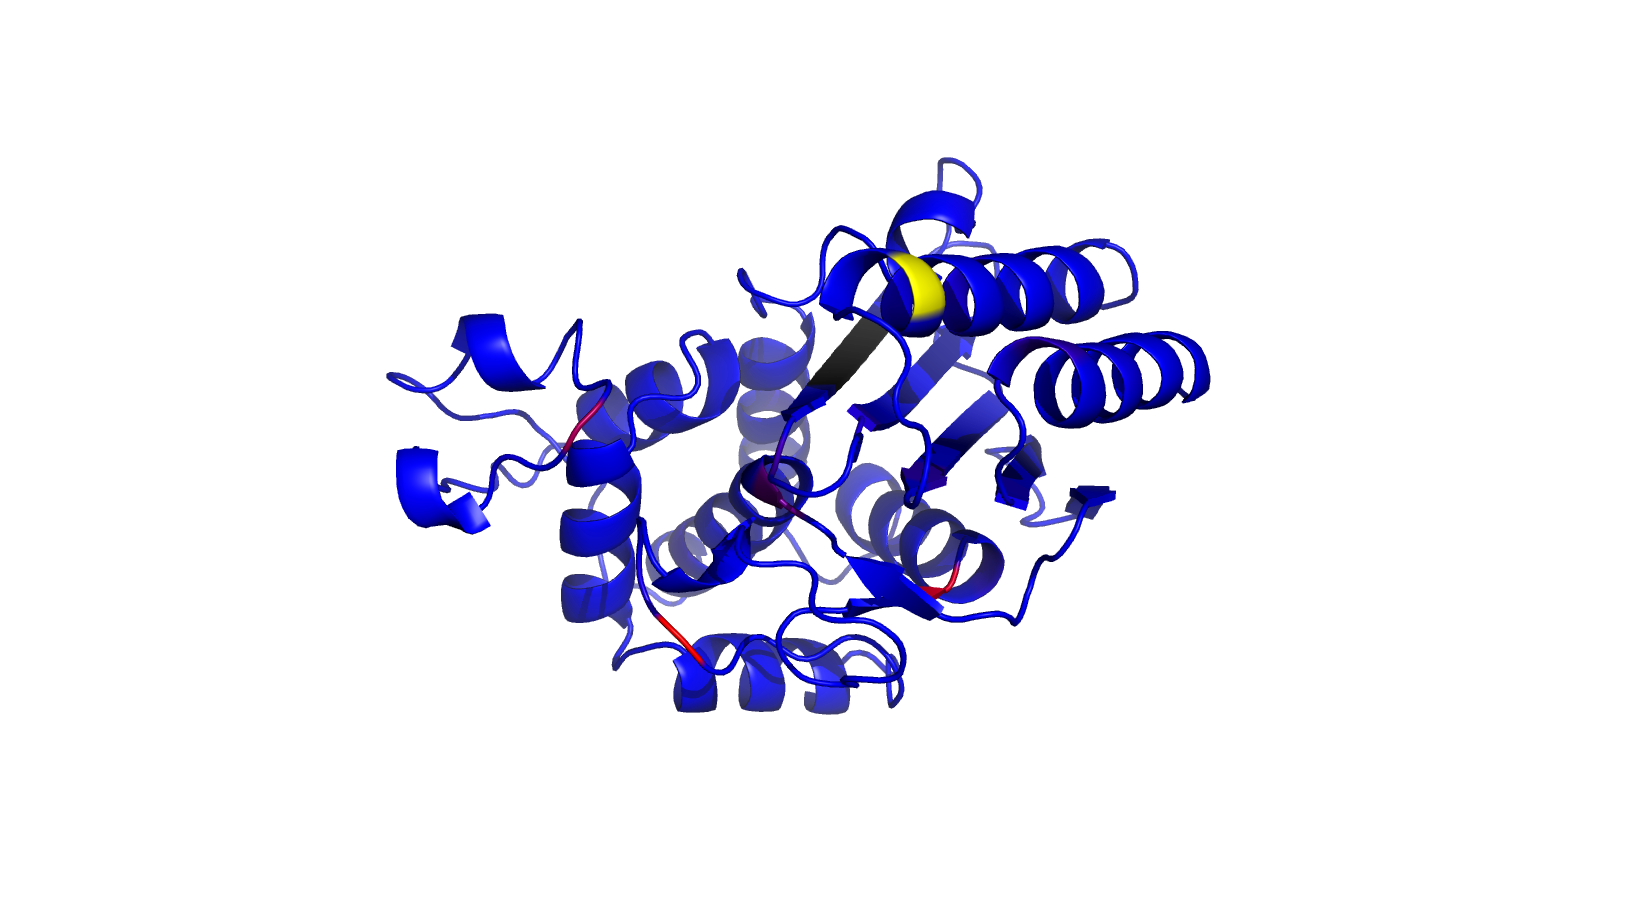
\includegraphics[width=\textwidth]{ch4/1xpb_GL.png}
	\caption{Distribution of genetic load in TEM mapped on its structure (1xpb). 
	Average genetic load over all observed TEM variants is indicated by the color, blue low genetic load, red high.}
	\label{fig:tem2016_3d}
\end{figure}


\begin{figure}[H]
     \centering
	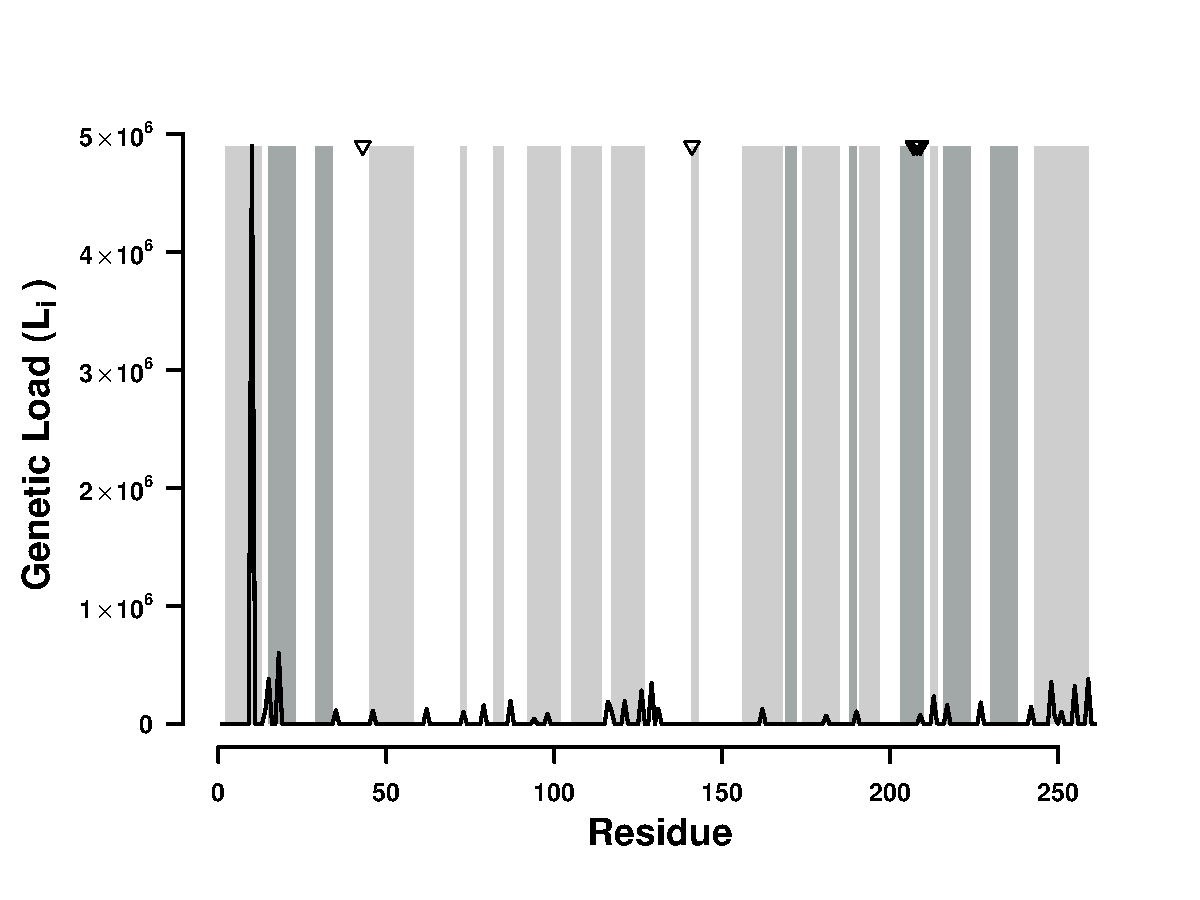
\includegraphics[width=\textwidth]{img/GL_slide_SHV2016}
	\caption{Distribution of genetic load in SHV. 
	Average genetic load over all observed SHV variants is indicated by the black line. 
	Light gray bars indicate where helices are found, and dark gray bars indicate $\beta$-sheets.
	The three residues forming the active sites are indicated by three triangles at the top of the plot.}
	\label{fig:shv2016_sse}
\end{figure}

\begin{figure}[h]
    \centering
    \begin{subfigure}
        \centering
        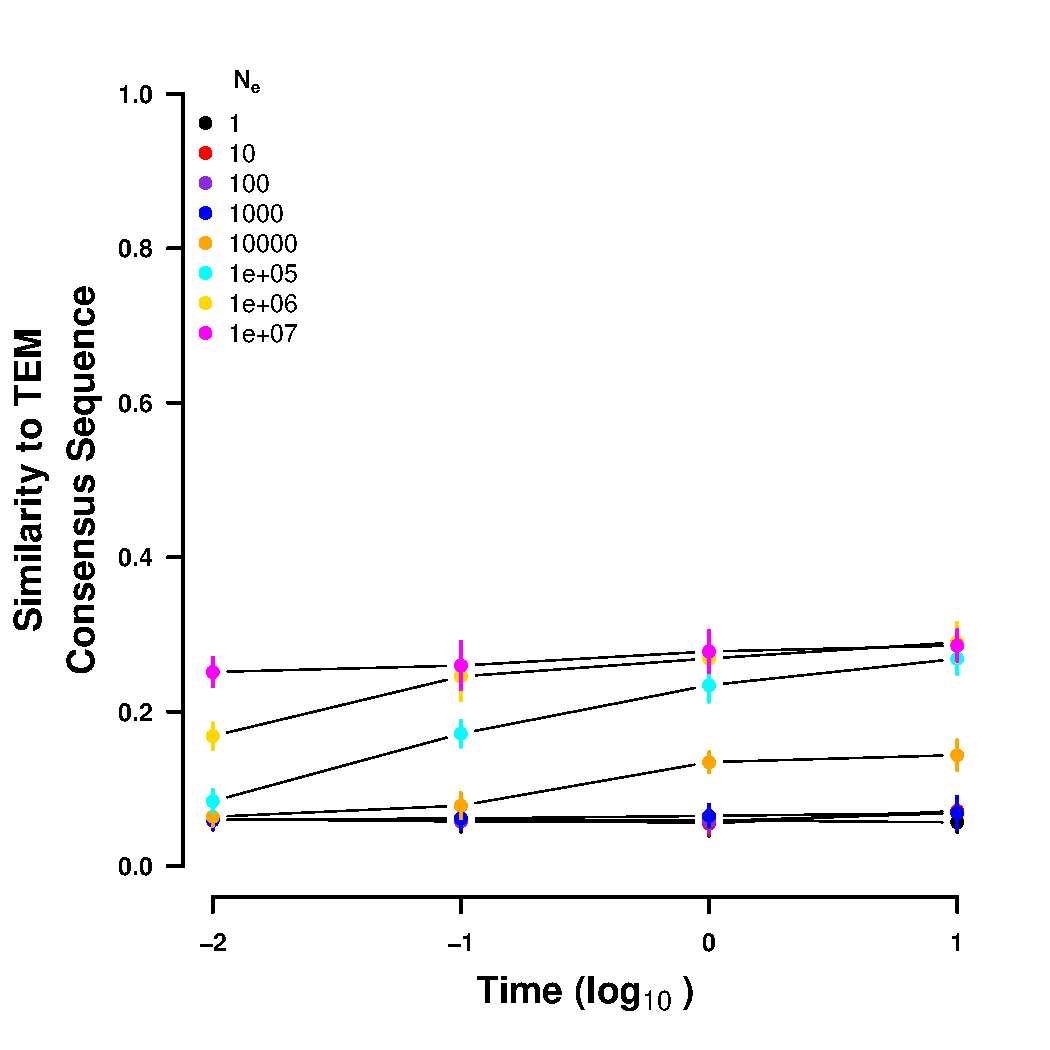
\includegraphics[width=.45\textwidth]{img/simulated_dist_time_SELAC_random.pdf}
    \end{subfigure}
    \begin{subfigure}
        \centering
        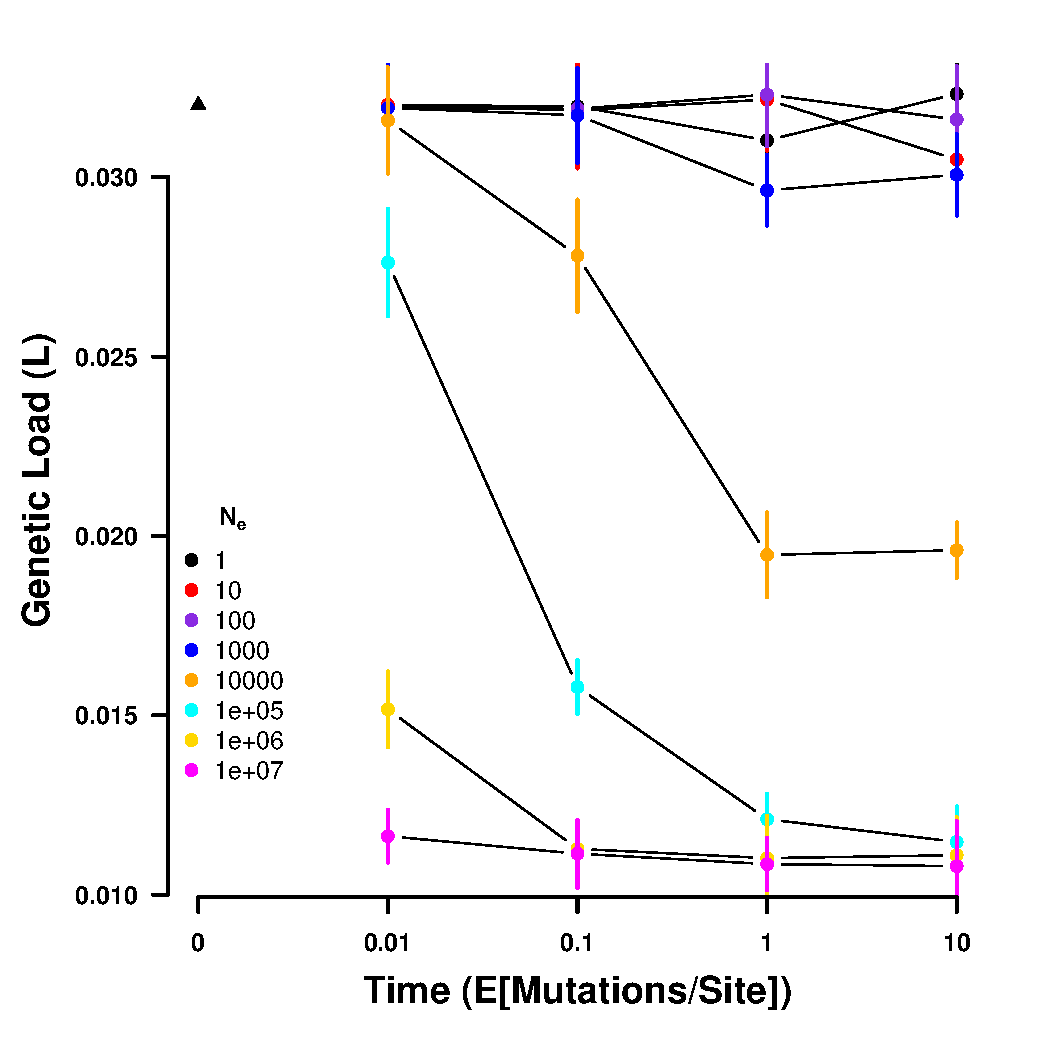
\includegraphics[width=.45\textwidth]{img/simulated_gl_time_SELAC_random.pdf}
    \end{subfigure}
    \caption{Sequences simulated from a random codon sequence under the site specific selection on amino acids estimated using \selac. 
    (left) Sequence similarity to the observed consensus sequence at various times for a range on values of $N_e$.
    (right) Genetic load of the simulated sequences at various times for a range on values of $N_e$.
    Time is given in number of expected mutations per site, which equals the substitution rate of a neutral mutation.
    Points indicate sample means and vertical bars indicate standard deviations. Initial sequence is the inferred ancestral state of the TEM variants and indicated by a black triangle.}
    \label{fig:selac_sim_rand}
\end{figure}

\begin{figure}[h]
    \centering
    \begin{subfigure}
        \centering
        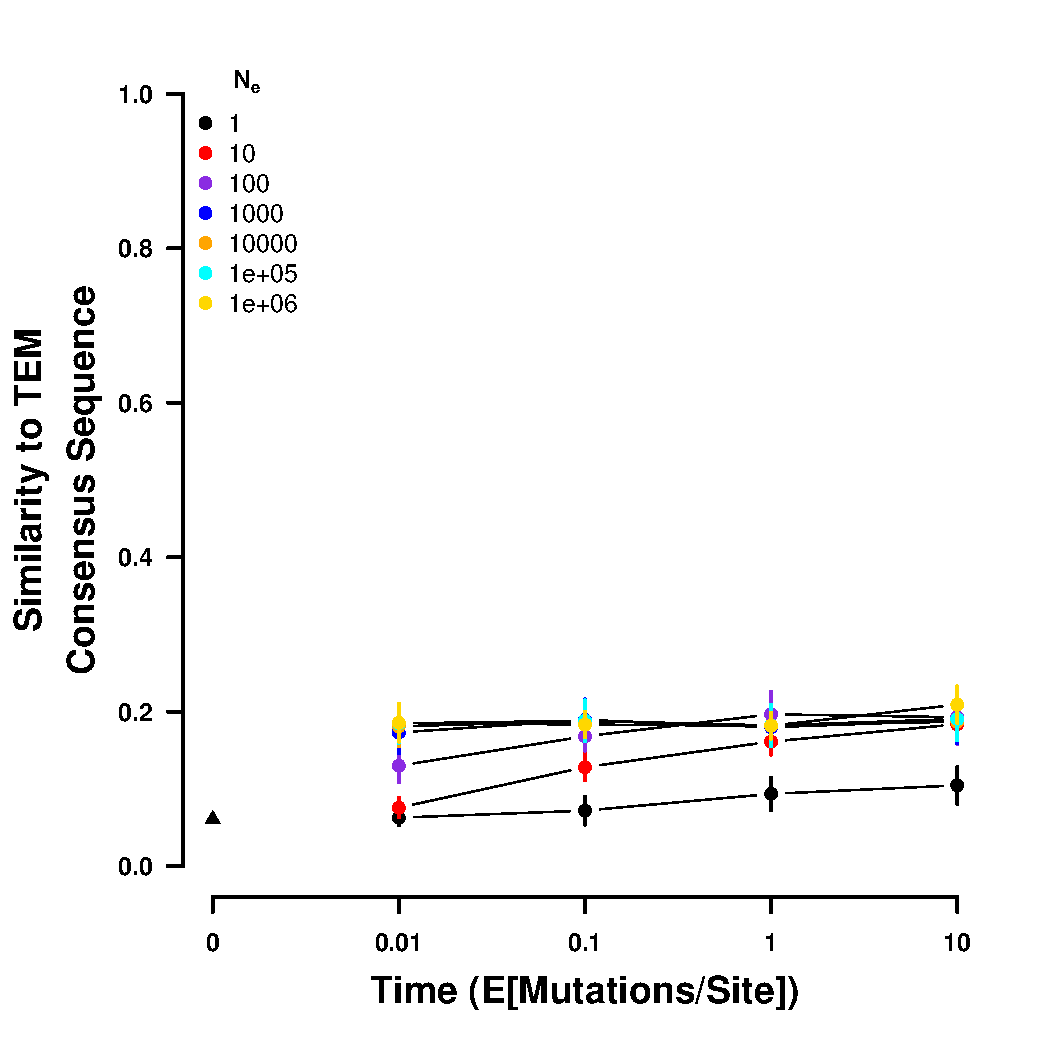
\includegraphics[width=.45\textwidth]{img/simulated_dist_time_DMS_random.pdf}
    \end{subfigure}
    \begin{subfigure}
        \centering
        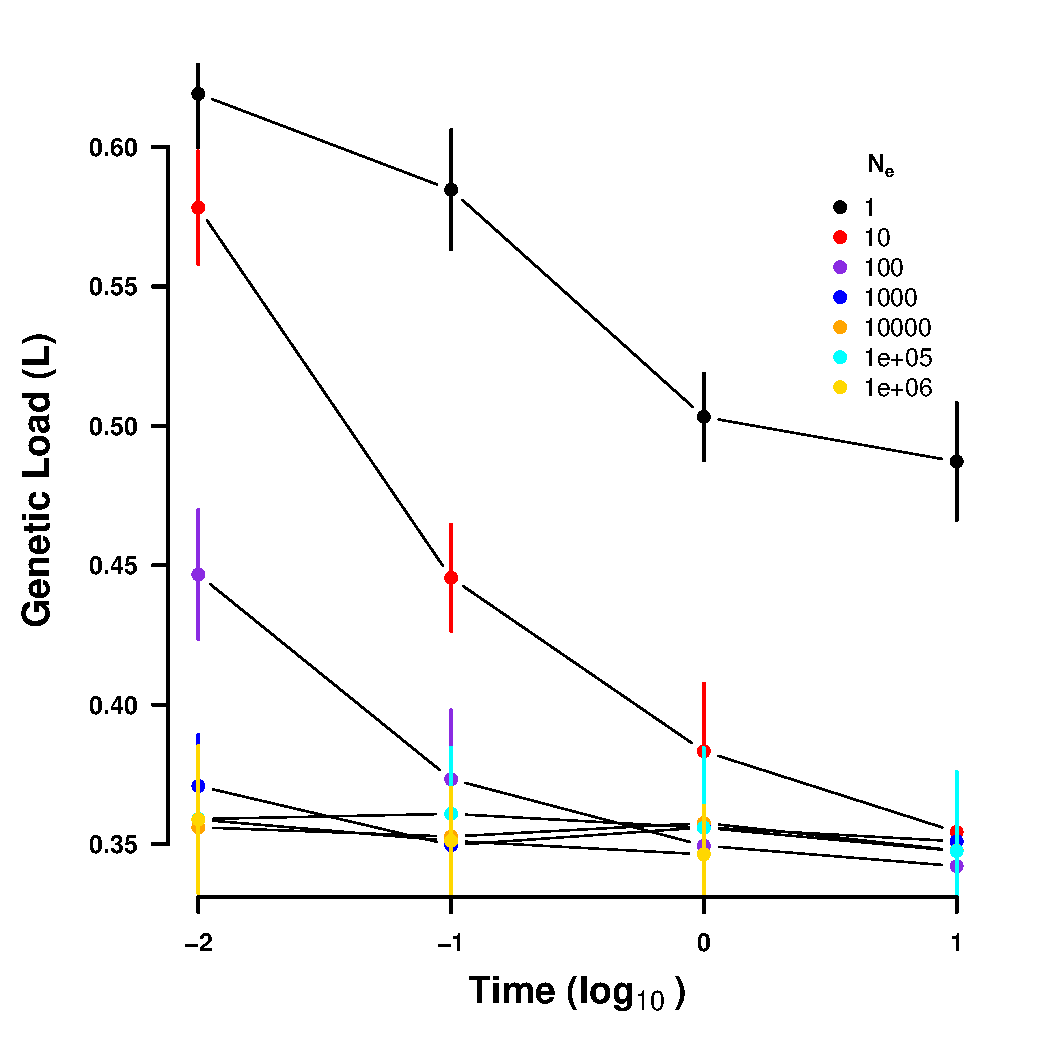
\includegraphics[width=.45\textwidth]{img/simulated_gl_time_DMS_random.pdf}
    \end{subfigure}
    \caption{Sequences simulated from a random codon sequence under the site specific selection on amino acids estimated using deep mutation scanning. 
    (left) Sequence similarity to the observed consensus sequence at various times for a range on values of $N_e$.
    (right) Genetic load of the simulated sequences at various times for a range on values of $N_e$.
    Time is given in number of expected mutations per site, which equals the substitution rate of a neutral mutation.
    Points indicate sample means and vertical bars indicate standard deviations. Initial sequence is the inferred ancestral state of the TEM variants and indicated by a black triangle.}
    \label{fig:dms_sim_rand}
\end{figure}

\begin{figure}[h]
    \centering
    \begin{subfigure}
        \centering
        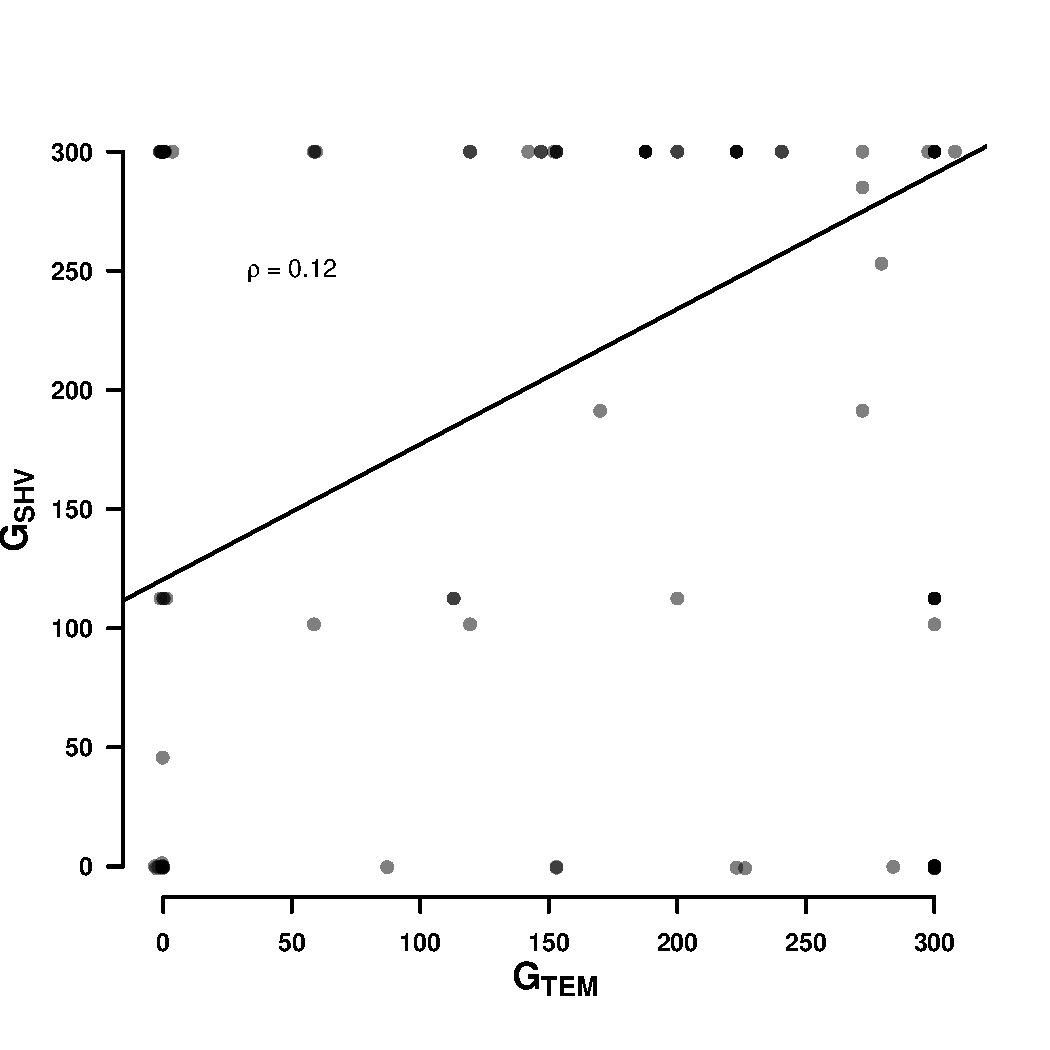
\includegraphics[width=.45\textwidth]{img/g_shift_lac.pdf}
    \end{subfigure}
    \begin{subfigure}
        \centering
        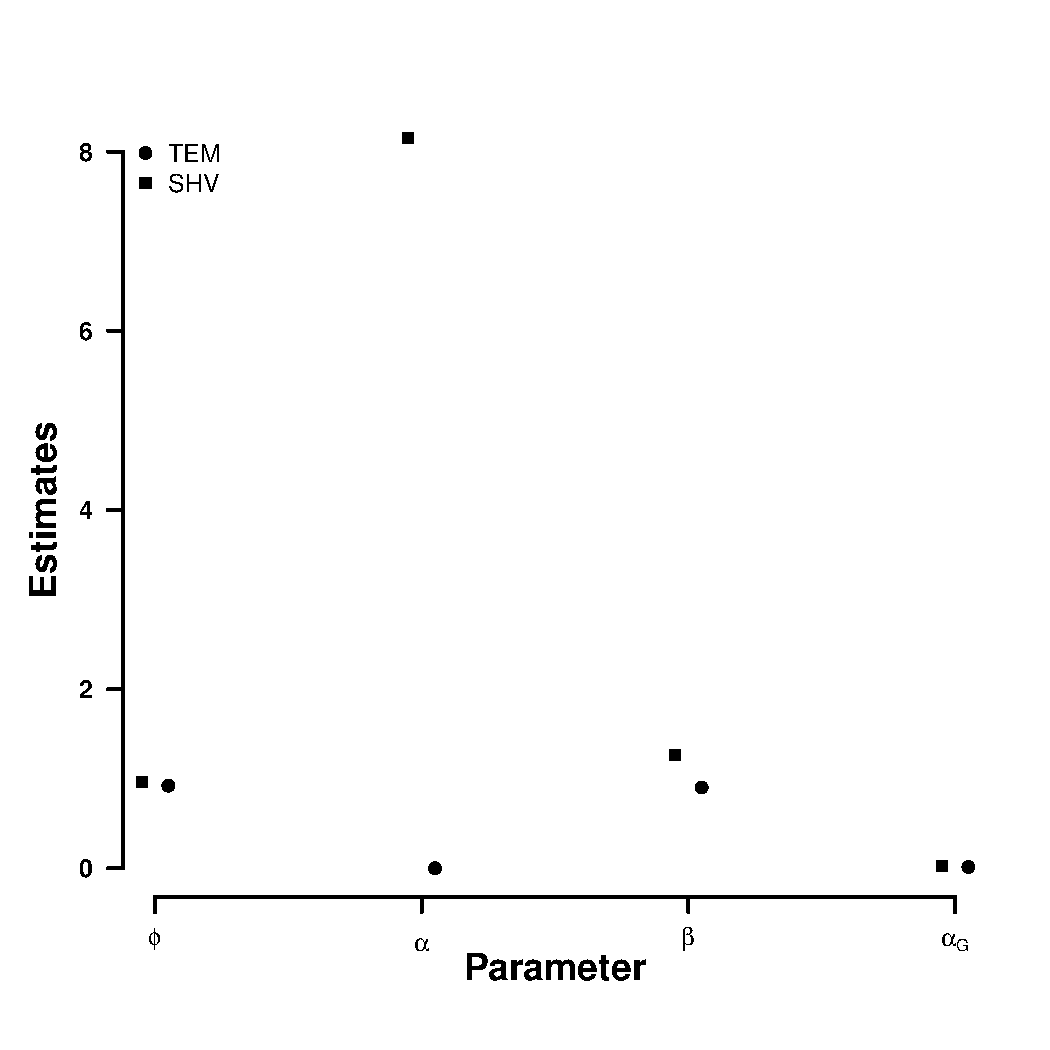
\includegraphics[width=.45\textwidth]{img/TEM_SHV_2016_par_comp.pdf}
    \end{subfigure}
    \caption{Comparison of selection related parameters between TEM and SHV. 
    (left) Estimated site specific efficacy of selection $G$. 
    (right) Selection related parameter estimates. 
    Protein functionality production rate $\psi$, \PC weight for amino acid composition $\alpha_c$, \PC weight for amino acid polarity $\alpha_p$, and the parameter describing the distribution of $G$, $\alpha_G$ estimated by \selac.}
    \label{fig:tem_shv_param_comp}
\end{figure}

\end{document}
